\documentclass[12pt,twosides,onecolumn,openany]{article}
\usepackage{graphicx} 

\usepackage{cite}
\usepackage[catalan]{babel}
\usepackage{emptypage}
\usepackage{hyperref}
\usepackage{mathtools}
\usepackage{blindtext}
\usepackage{subfigure}
\usepackage[utf8]{inputenc}
\usepackage{caption}
\usepackage{subcaption}
\usepackage{wrapfig}
\usepackage[a4paper]{geometry}
\geometry{top=2.5cm, bottom=2.5cm, left=2.5cm, right=2.5cm}
\usepackage{fancyhdr}
\pagestyle{fancy}
\usepackage{amsmath}
\usepackage{amssymb}
\usepackage{amsfonts}
\providecommand{\norm}[1]{\lVert#1\rVert}
\hypersetup{colorlinks=true,urlcolor=blue,linkcolor=blue}
\usepackage{multirow}
\usepackage{multicol}
\usepackage{rotating}

\usepackage{titlesec}

\newenvironment{Figura}
  {\par\medskip\noindent\minipage{\linewidth}}
  {\endminipage\par\medskip}

\titleformat{\section}  % comando de sección a formatear
  {\fontsize{14}{16}\bfseries} % formato para toda la línea
  {\thesection} % cómo mostrar el número
  {0.4em} % espacio entre el número y el texto
  {} % formato solo para el texto
  [] % formato para después del texto


\fancyhf{}
\fancyhead[LO,RE]{Grup D3}
\fancyhead[RO,LE]{Pràctica Ib}
\fancyfoot[LO,RE]{\thepage}
\fancyfoot[RO,LE]{Laboratori de Termodinàmica - UAB}
\graphicspath{ {images/} }

\begin{document}

\begin{center}
    {\Large \textsc{Transport de la calor: Comprovació de la llei de Stefan}}\\
    \vspace{0.2cm}
    \textsc{30 d'Octubre de 2024}\\
    \vspace{0.2cm}
    $\begin{matrix} 
    \text{Miguel A.} \hspace{1.5cm} & \text{Daniel B.} & \hspace{1.5cm} \text{Sergi R.}\\1637738 \hspace{1.5cm} & 1603508 & \hspace{1.5cm} 1607805
    \end{matrix}$
\end{center}
\begin{center}
    \textsc{\textit{RESUM}}
\end{center}
En aquesta pràctica de laboratori s'estudien els fenòmens de transport de calor que participen en una bombeta de tungstè. A partir de mesures indirectes es mostra la convivència entre el fenomen de la convecció i el de la radiació quan la bombeta emet energia en forma de calor. A partir de l'equació de calor de Newton i la llei de Stefan-Boltzmann es posa de manifest la conservació de l'energia a l'estudiar quina relació tenen amb la potència elèctrica aportada a la bombeta. Finalment, es comprova a partir de mesures directes de la radiació emesa per la bombeta que es compleix la llei de Stefan-Boltzmann.
\vspace{0.5cm}
\begin{multicols}{2}
\section{Introducció i objectius}
Per a qualsevol circuit senzill com el d'una bombeta connectada al corrent podem veure que es compleix la relació
\begin{equation}\label{Pot_elec}
  P_{\text{e}} = VI
\end{equation}
on $P_{\text{e}}$ és la potència elèctrica, $V$ el potencial elèctric i $I$ la intensitat de corrent, per a obtenir la potència elèctrica subministrada; i la relació
\begin{equation}\label{Llei_Ohm}
  V =IR
\end{equation}
coneguda com la llei d'Ohm, on $R$ és la resistència elèctrica del sistema. Durant aquesta experiència treballarem amb una bombeta de tungstè de \(220 \, \text{V}\) i dues fonts de voltatge diferents: una DC i l'altra AC. Considerarem que la resistència elèctrica del tungstè seguirà un comportament lineal amb la temperatura, és a dir
\begin{equation}\label{resistencia}
  R = R_0[1+\alpha\Delta T]
\end{equation}
on $\Delta T = (T - T_a)$ és la diferència de temperatures respecte a la temperatura ambient del laboratori, $R_0$ el valor de la resistència a temperatura ambient i $\alpha$ és el coeficient mitjà de temperatura del filament de tungstè, aquest coeficient pren un valor\footnote{Durant aquesta pràctica hem fet servir aquest valor de $\alpha$, però es pot fer recerca a la literatura del seu valor. D'entre altres, el coeficient mitjà del tungstè pot prendre el valor de \(\bar{\alpha}_1 = 0,0053\,\text{K}^{-1}\) \cite{llibre_lab} o de \( \bar{\alpha}_2 = 0,0045\, \text{K}^{-1}\) \cite{toolbox}} de \(\alpha = 0,0048 \, \text{K}^{-1}\).
El nostre objectiu és estudiar el comportament de la transmissió de la calor a través de diferents processos. Analitzant el sistema bombeta-entorn, podem deduir que només seran significatius dos processos d'intercanvi de calor. El primer d'ells és la convecció, regida per l'equació de Newton:
\begin{equation}\label{Newton}
  P_{\text{c}} = -\lambda A\Delta T
\end{equation}
on $\lambda$ és el coeficient de convecció i $A$ l'àrea del sistema en contacte amb l'aire. Per a realitzar els nostres càlculs ens interessarà treballar amb el logaritme d'aquesta equació
\begin{equation}\label{ln_Newton}
  \ln{P_{\text{c}}} = \ln{\Delta T} + \ln{(-\lambda A)}
\end{equation}
Notem que es prediu un comportament lineal de pendent 1 respecte $\ln{\Delta T}$. El segon procés d'intercanvi de calor que participa és la radiació, regida per la llei de Stefan-Boltzmann
\begin{equation}\label{Stefan_Boltzmann}
  P_{\text{r}} = e\sigma_{\text{SB}}AT^{4}
\end{equation}
on $e$ és l'emissivitat i $\sigma_{\text{SB}}$ és la constant d'Stefan-Boltzmann, que pren el valor \(\sigma_{\text{SB}} = (5,6697\pm0,0029) \, \text{W}/\text{m}^{2}\text{K}^{4}\) \cite{guia_lab}. Novament, ens interessa treballar amb el logaritme, que en aquest cas prediu també un comportament lineal però aquest cop de pendent 4:
\begin{equation}\label{ln_Stefan_Boltzmann}
  \ln{P_{\text{r}}} = 4\ln{T} + \ln{(e\sigma_{\text{SB}}A)}
\end{equation}
Es podria afegir com a darrer procés de transmissió de calor la conducció, però, aquest fenomen és gairebé exclusiu de la matèria condensada. El nostre sistema per on es pot transmetre calor es compon principalment per l'entorn (aire) i l'interior de la bombeta (buit). Pot existir aportació per part de la conducció, però en aquest cas la considerem negligible. Tenint tot això en compte, podem escriure el balanç energètic igualant la potència emesa amb la dispersada:
\begin{equation}\label{relacions_pot}
  P_{\text{e}}=P_{\text{c}} + P_{\text{r}}
\end{equation}
Cal notar que segons les Equacions \eqref{Newton} i \eqref{Stefan_Boltzmann} podem esperar dels nostres resultats que a baixes tensions, és a dir a baixa temperatura, estarà poc pressent la contribució de radiació ($\sigma_{\text{SB}}$ és molt petita), mentre que a altes tensions, alta temperatura, serà molt pressent (hi ha un creixement quàrtic).
\section{Resultats i discussió}
Per a poder obtenir les dades corresponents a $\Delta T$ és necessari obtenir el valor de la temperatura ambient al laboratori. Però, aquesta no ha sigut constant al llarg de tota l'experiència, per tant, treballarem amb un valor mitjà obtingut de diverses mesures fetes al llarg de l'experiència (veure Annex). El valor de la temperatura ambient que farem servir és: \(T_a = (297,8\pm0,2)\,\text{K} \).\\\\
Com a altra acció prèvia a realitzar l'experiència mesurem, a temperatura ambient, el valor de la resistencia $R_0$, obtenint el següent valor: \(R_0=(49,1\pm0,1)\,\Omega\). Finalment, com a darrera consideració a l'hora de realitzar els càlculs, calculem $R$ segons \eqref{Llei_Ohm} i a més afegim la resistència mitjana del cablejat, que pren un valor aproximat de \(0,8 \, \Omega\). Apliquem aquesta correcció per a poder calcular correctament la temperatura a partir de \eqref{resistencia}.
\subsection{Mesura indirecta}
A partir de les dades experimentals recollides obtenim la Figura \ref{fig:P_vs_R} i la Figura \ref{fig:lnP_vs_lnDeltaT}.
\begin{Figura}
  \centering
  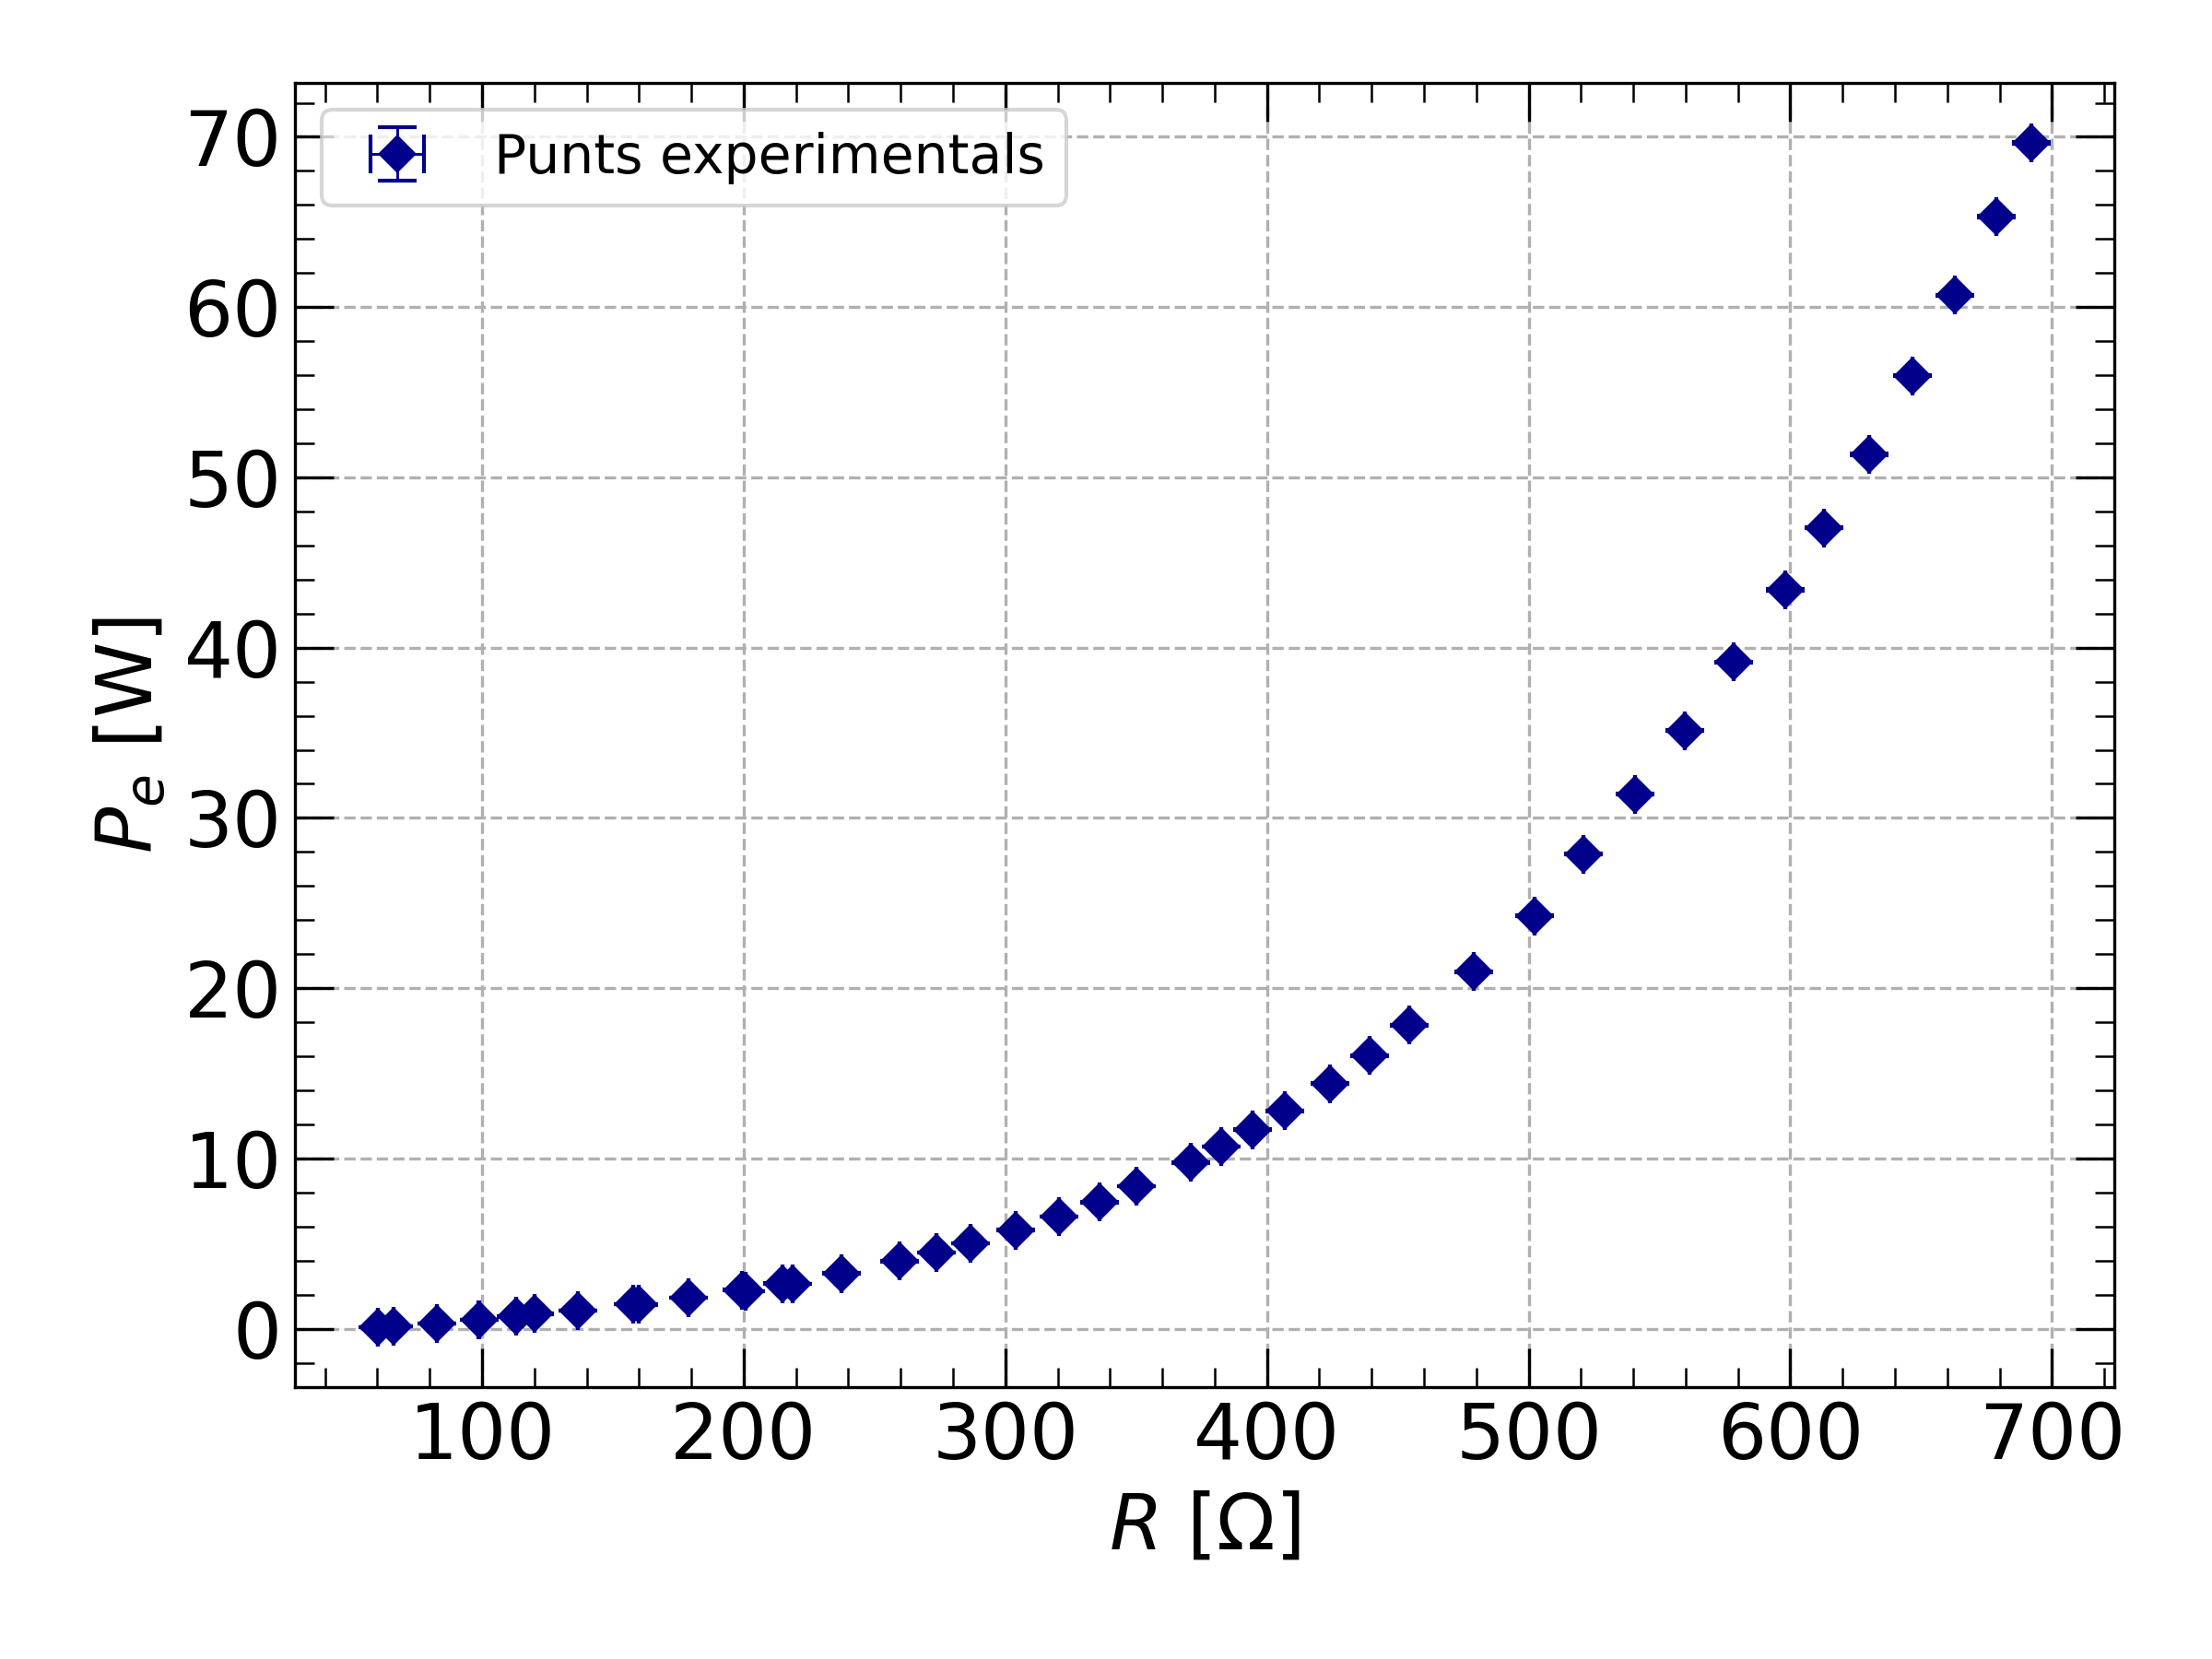
\includegraphics[width=\linewidth]{../../graphs/practica_Ib/plots/P_vs R.png}
  \captionof{figure}{\footnotesize{Representació de la potència elèctrica aplicada $P_{\text{e}}$ vs la resistència del filament de tungstè $R$.}}
  \label{fig:P_vs_R}
\end{Figura}
\begin{Figura}
  \centering
  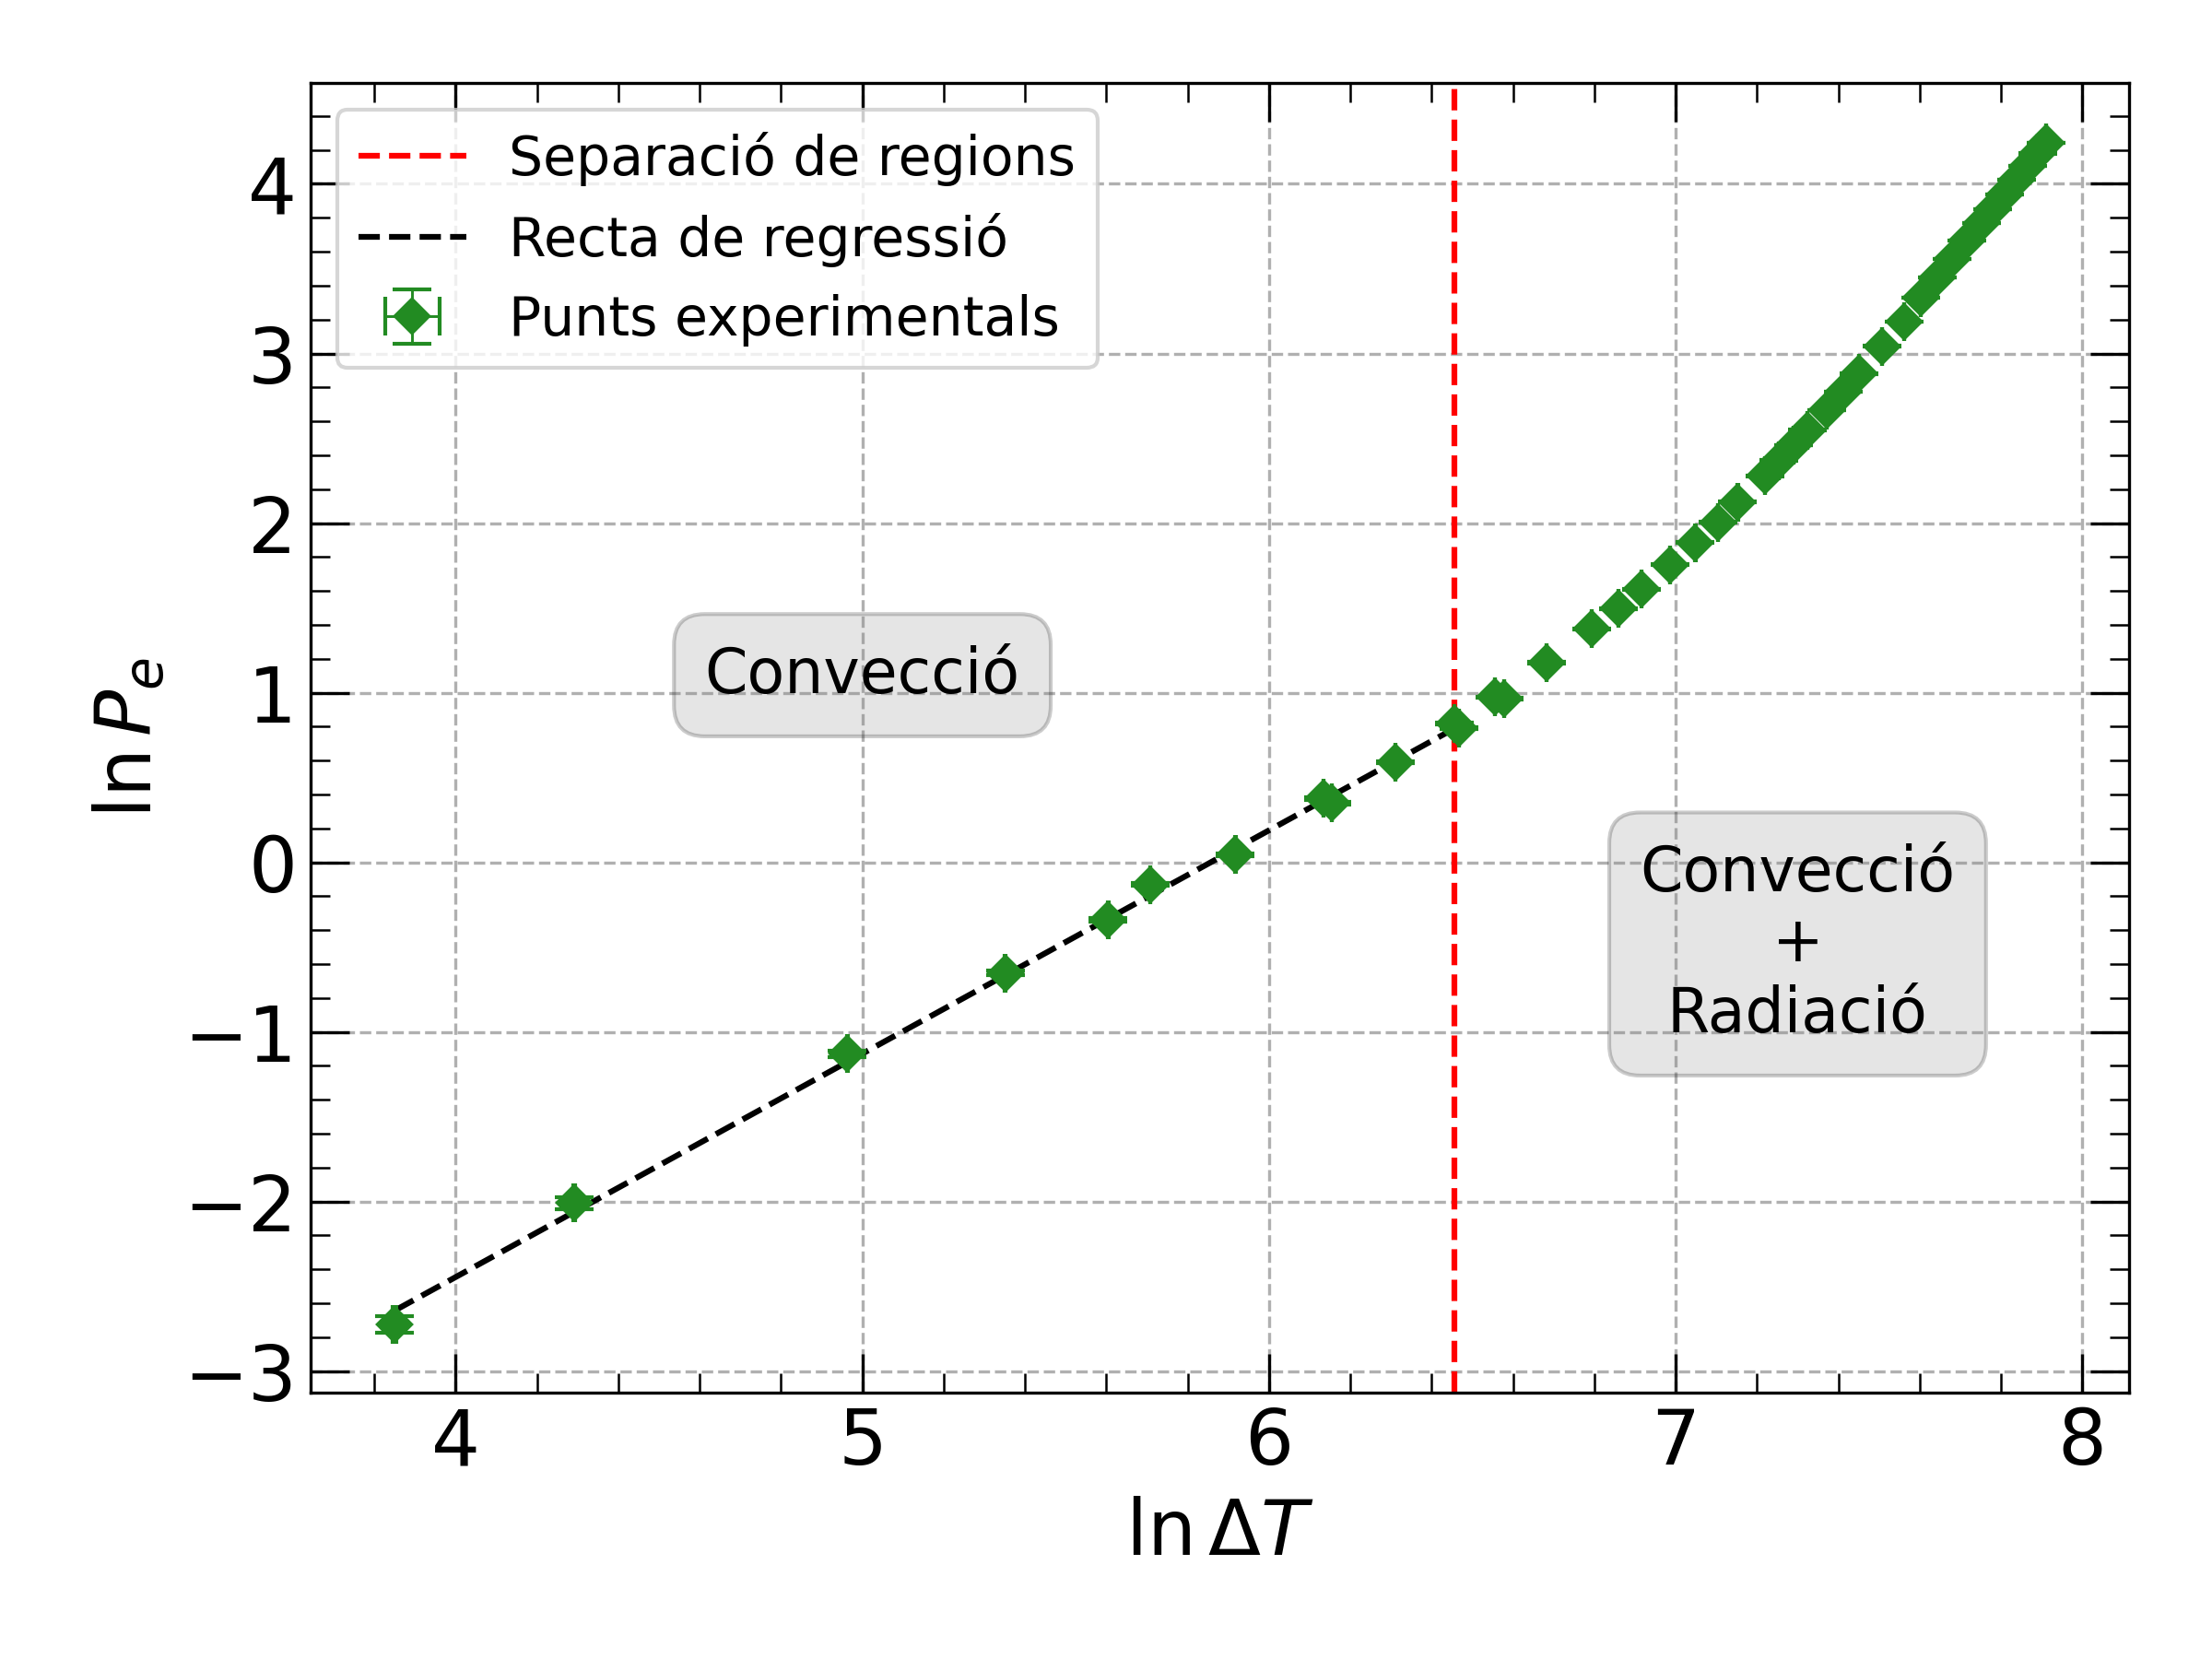
\includegraphics[width=\linewidth]{../../graphs/practica_Ib/plots/lnP_el_vs_lnT.png}
  \captionof{figure}{\footnotesize{Representació de $\ln{P_{\text{e}}}$ vs. $\ln{\Delta T}$. S'observen dues regions, separades per una línia vertical vermella. La primera regió (esquerra) participa majoritàriament la convecció, la segona (dreta) participen tant la convecció com la radiació. També es pot observar la regressió lineal ($y=ax+b$) de la primera regió. Coeficients de regressió: $a = 1,317 \pm 0,017$, $b = -7,71\pm0,10$. Regressió amb un coeficient de $r^2 = 0,999$.}}
  \label{fig:lnP_vs_lnDeltaT}
\end{Figura}
A la Figura \ref{fig:lnP_vs_lnDeltaT} s'observen dues zones diferents, una amb comportament lineal i una altra amb un comportament diferent. Agafant punt a punt i de forma ordenada (de $\Delta T$ menor a major) valors experimentals representats a la Figura \ref{fig:lnP_vs_lnDeltaT} fem diverses regressions lineals de forma iterada fins a obtenir el valor més gran per al coeficient de regressió $r^2$, obtenint el valor 11 com a nombre òptim de punts. Es pot veure representada a la mateixa Figura \ref{fig:lnP_vs_lnDeltaT} la regressió lineal obtinguda amb la llista de punts resultants.\\\\
Com es pot veure a l'Equació \eqref{ln_Newton} el pendent d'aquesta regressió hauria de ser $a=1$ si al sistema només s'intercanviés calor per convecció. Però, les dades obtingudes porten a deduir que aquesta hipòtesi inicial és incorrecta, és a dir, tot i ser petita, existeix una contribució de calor per radiació.\\\\
Podem realitzar una comprovació indirecta d'aquest resultat intentant calcular $R_0$ a partir d'extrapolar les nostres dades. Si assumim novament que a la primera regió participa de forma exclusiva la convecció veiem com, per a un rang baix de temperatures i seguint l'Equació \eqref{Newton} i l'Equació \eqref{resistencia}, la potència elèctrica hauria de tenir un comportament lineal amb la resistència. Aquest comportament lineal es pot observar als primers punts de la Figura \ref{fig:P_vs_R}.\\\\
Seleccionem els primers punts experimentals de manera que al fer una regressió obtenim un coeficient $r^2$ satisfactori. A partir dels coeficients obtinguts extrapolem el valor de $\tilde{R}_0$, el valor de la resistnècia quan no hi ha potència elèctrica, que a temperatura ambient hauria de coincidir amb el valor mesurat. Podem observar les dades escollides i la seva corresponent regressió lineal a la Figura \ref{fig:reg_P_vs_R}.\\\\
El valor extrapolat de la resistència obtingut és
\begin{equation*}
  \tilde{R}_0 = (55,34\pm0,03)\,\Omega
\end{equation*}
Veiem com $\tilde{R}_0$, tot i ser a prop del valor mesurat de $R_0$ es queda lluny d'entrar dins de la incertesa obtinguda. Podem interpretar novament aquest resultat suposant que la hipòtesi inicial, on assumim l'exclusivitat de la convecció en l'intercanvi de calor, és errònia.
\begin{Figura}
  \centering
  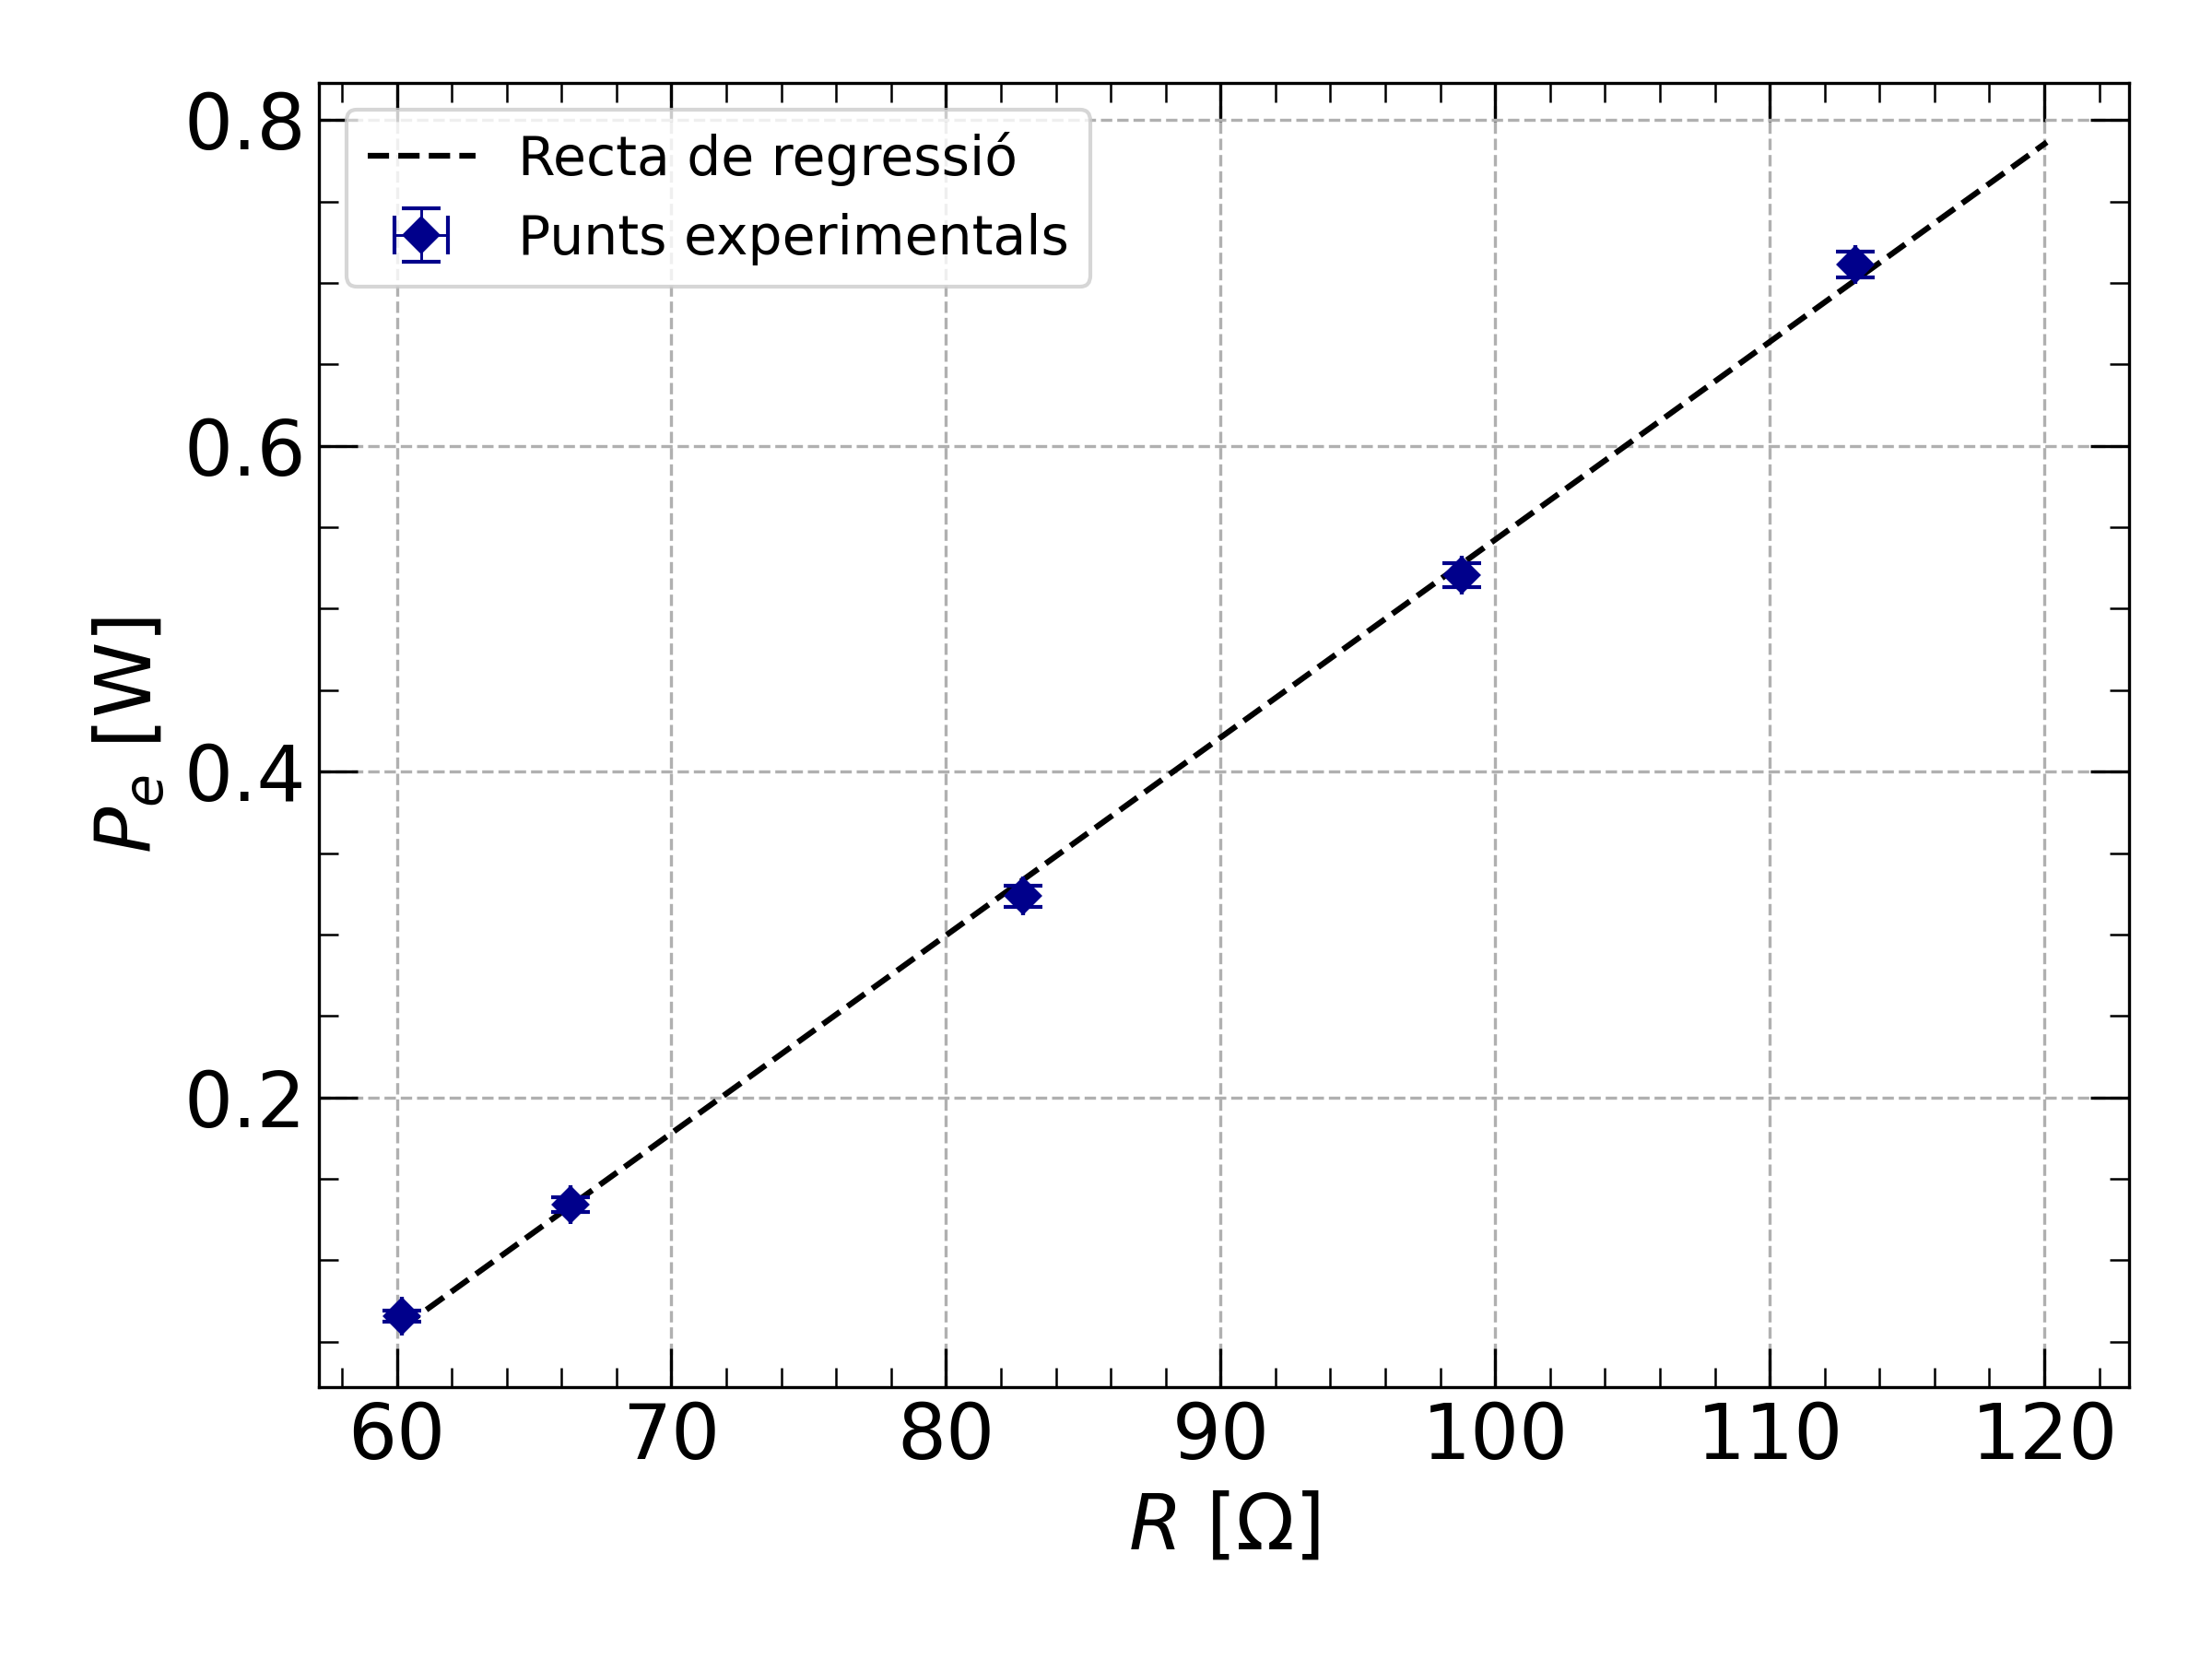
\includegraphics[width=\linewidth]{../../graphs/practica_Ib/plots/reg_P_vs_R.png}
  \captionof{figure}{\footnotesize{Representació i regressió lineal ($y =ax +b$) dels primers cinc punts experimentals de la gràfica $P_{\text{e}}$ vs. $R$. Coeficients de regressió: \(a=(12,1\pm0,2)\cdot10^{-3}\,\text{W}/\Omega\), \(b = (-0,672\pm0,019) \, \text{W}\). Regressió amb un coeficient de $r^2 =0,999$.}}
  \label{fig:reg_P_vs_R}
\end{Figura}
Tenint en compte l'Equació \eqref{relacions_pot} podem calcular la contribució per radiació a la segona regió marcada a la Figura \ref{fig:lnP_vs_lnDeltaT} restant als valors experimentals. Per a fer això podem, a partir de les dades de regressió de la Figura \ref{fig:lnP_vs_lnDeltaT}, extrapolar els punts necessaris i fer la resta. Podem observar amb més detall la segona regió i l'extrapolació a la Figura \ref{extrapolacio}. Es pot notar com la diferència entre la predicció de la convecció i els valors experimentals augmenta més i més a mesura que la diferència de temperatura també augmenta.
\begin{Figura}
  \centering
  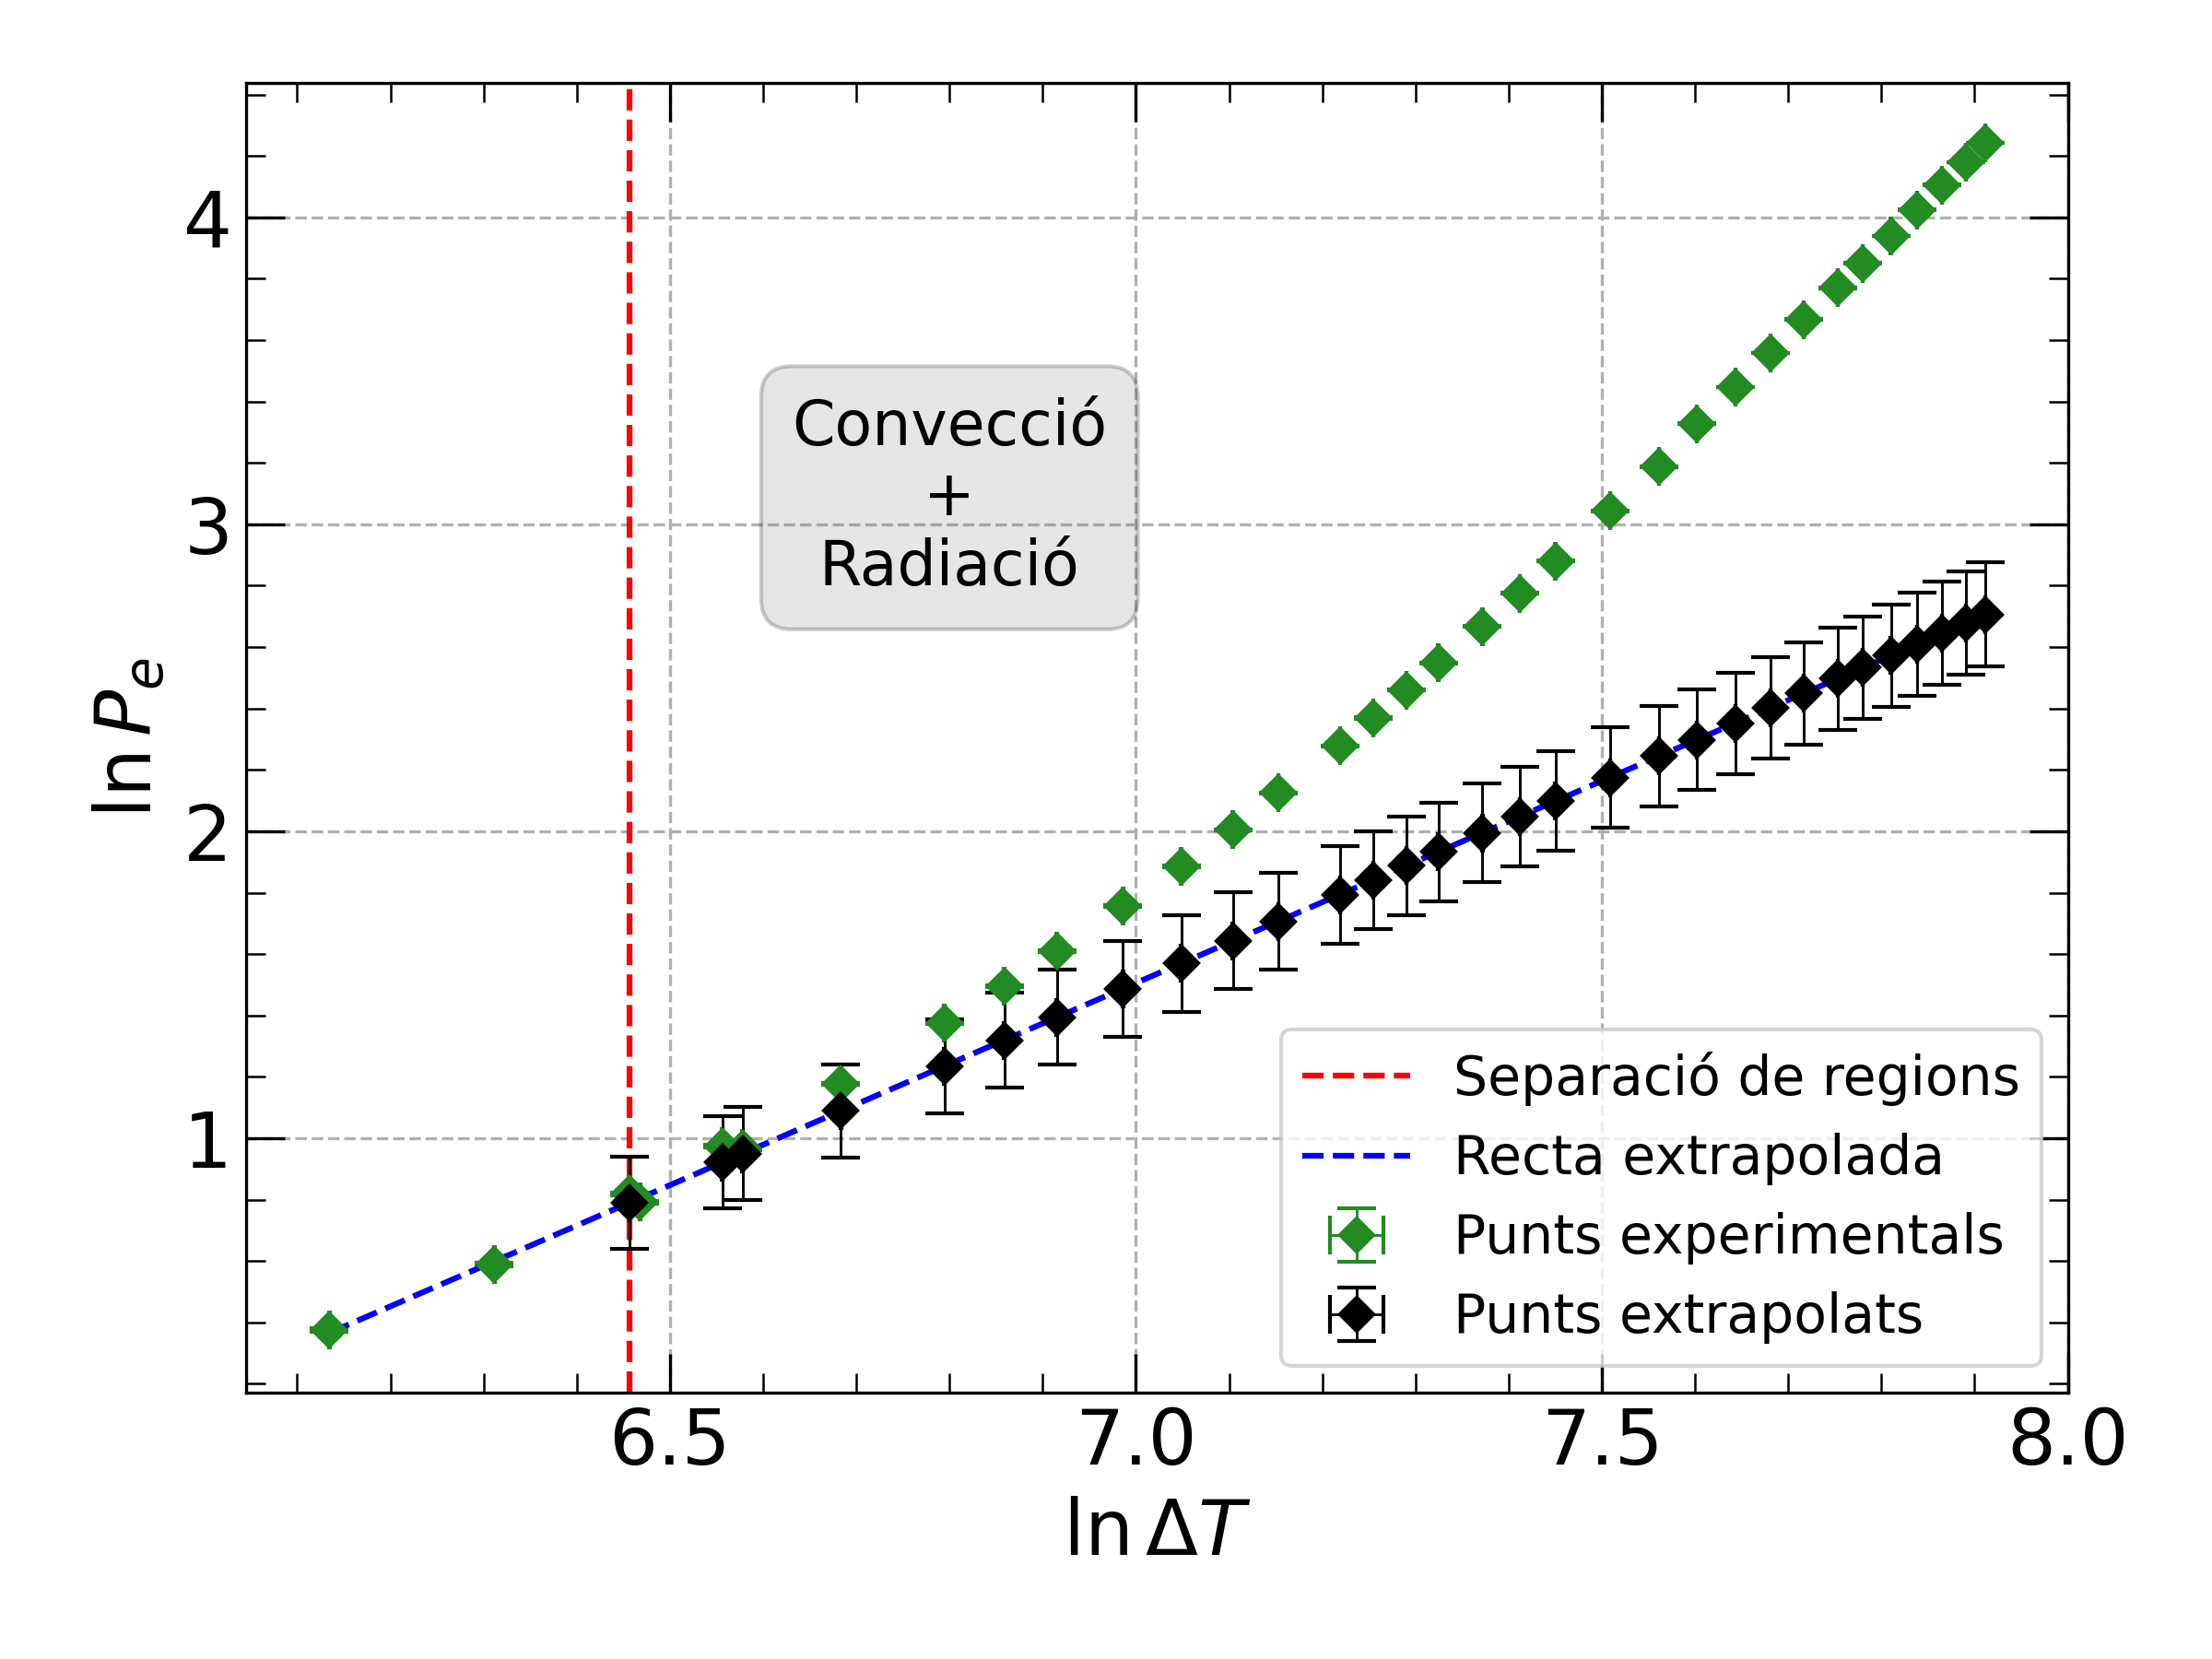
\includegraphics[width=\linewidth]{../../graphs/practica_Ib/plots/extrapolació.png}
  \captionof{figure}{\footnotesize{Representació de la segona regió de la gràfica $\ln{P_{\text{e}}}$ vs. $\ln{\Delta T}$ i extrapolació de la recta de convecció.}}
  \label{extrapolacio}
\end{Figura}
Amb aquest conjunt de dades $\ln{P_{\text{e}}}$ i $\ln{P_{\text{c}}}$ a la regió de la dreta recalculem els valors $P_{\text{e}}$ i $P_{\text{c}}$ corresponents i apliquem l'Equació \eqref{relacions_pot}. Amb el resultat tornem a graficar els logaritmes, obtenint la Figura \ref{fig:lnP_rad_vs_ln_T}. Notem com s'ha graficat respecte a $T$ i no respecte a $\Delta T$ per a obtenir una dependència que correspongui amb la llei de Stefan.
\begin{Figura}
  \centering
  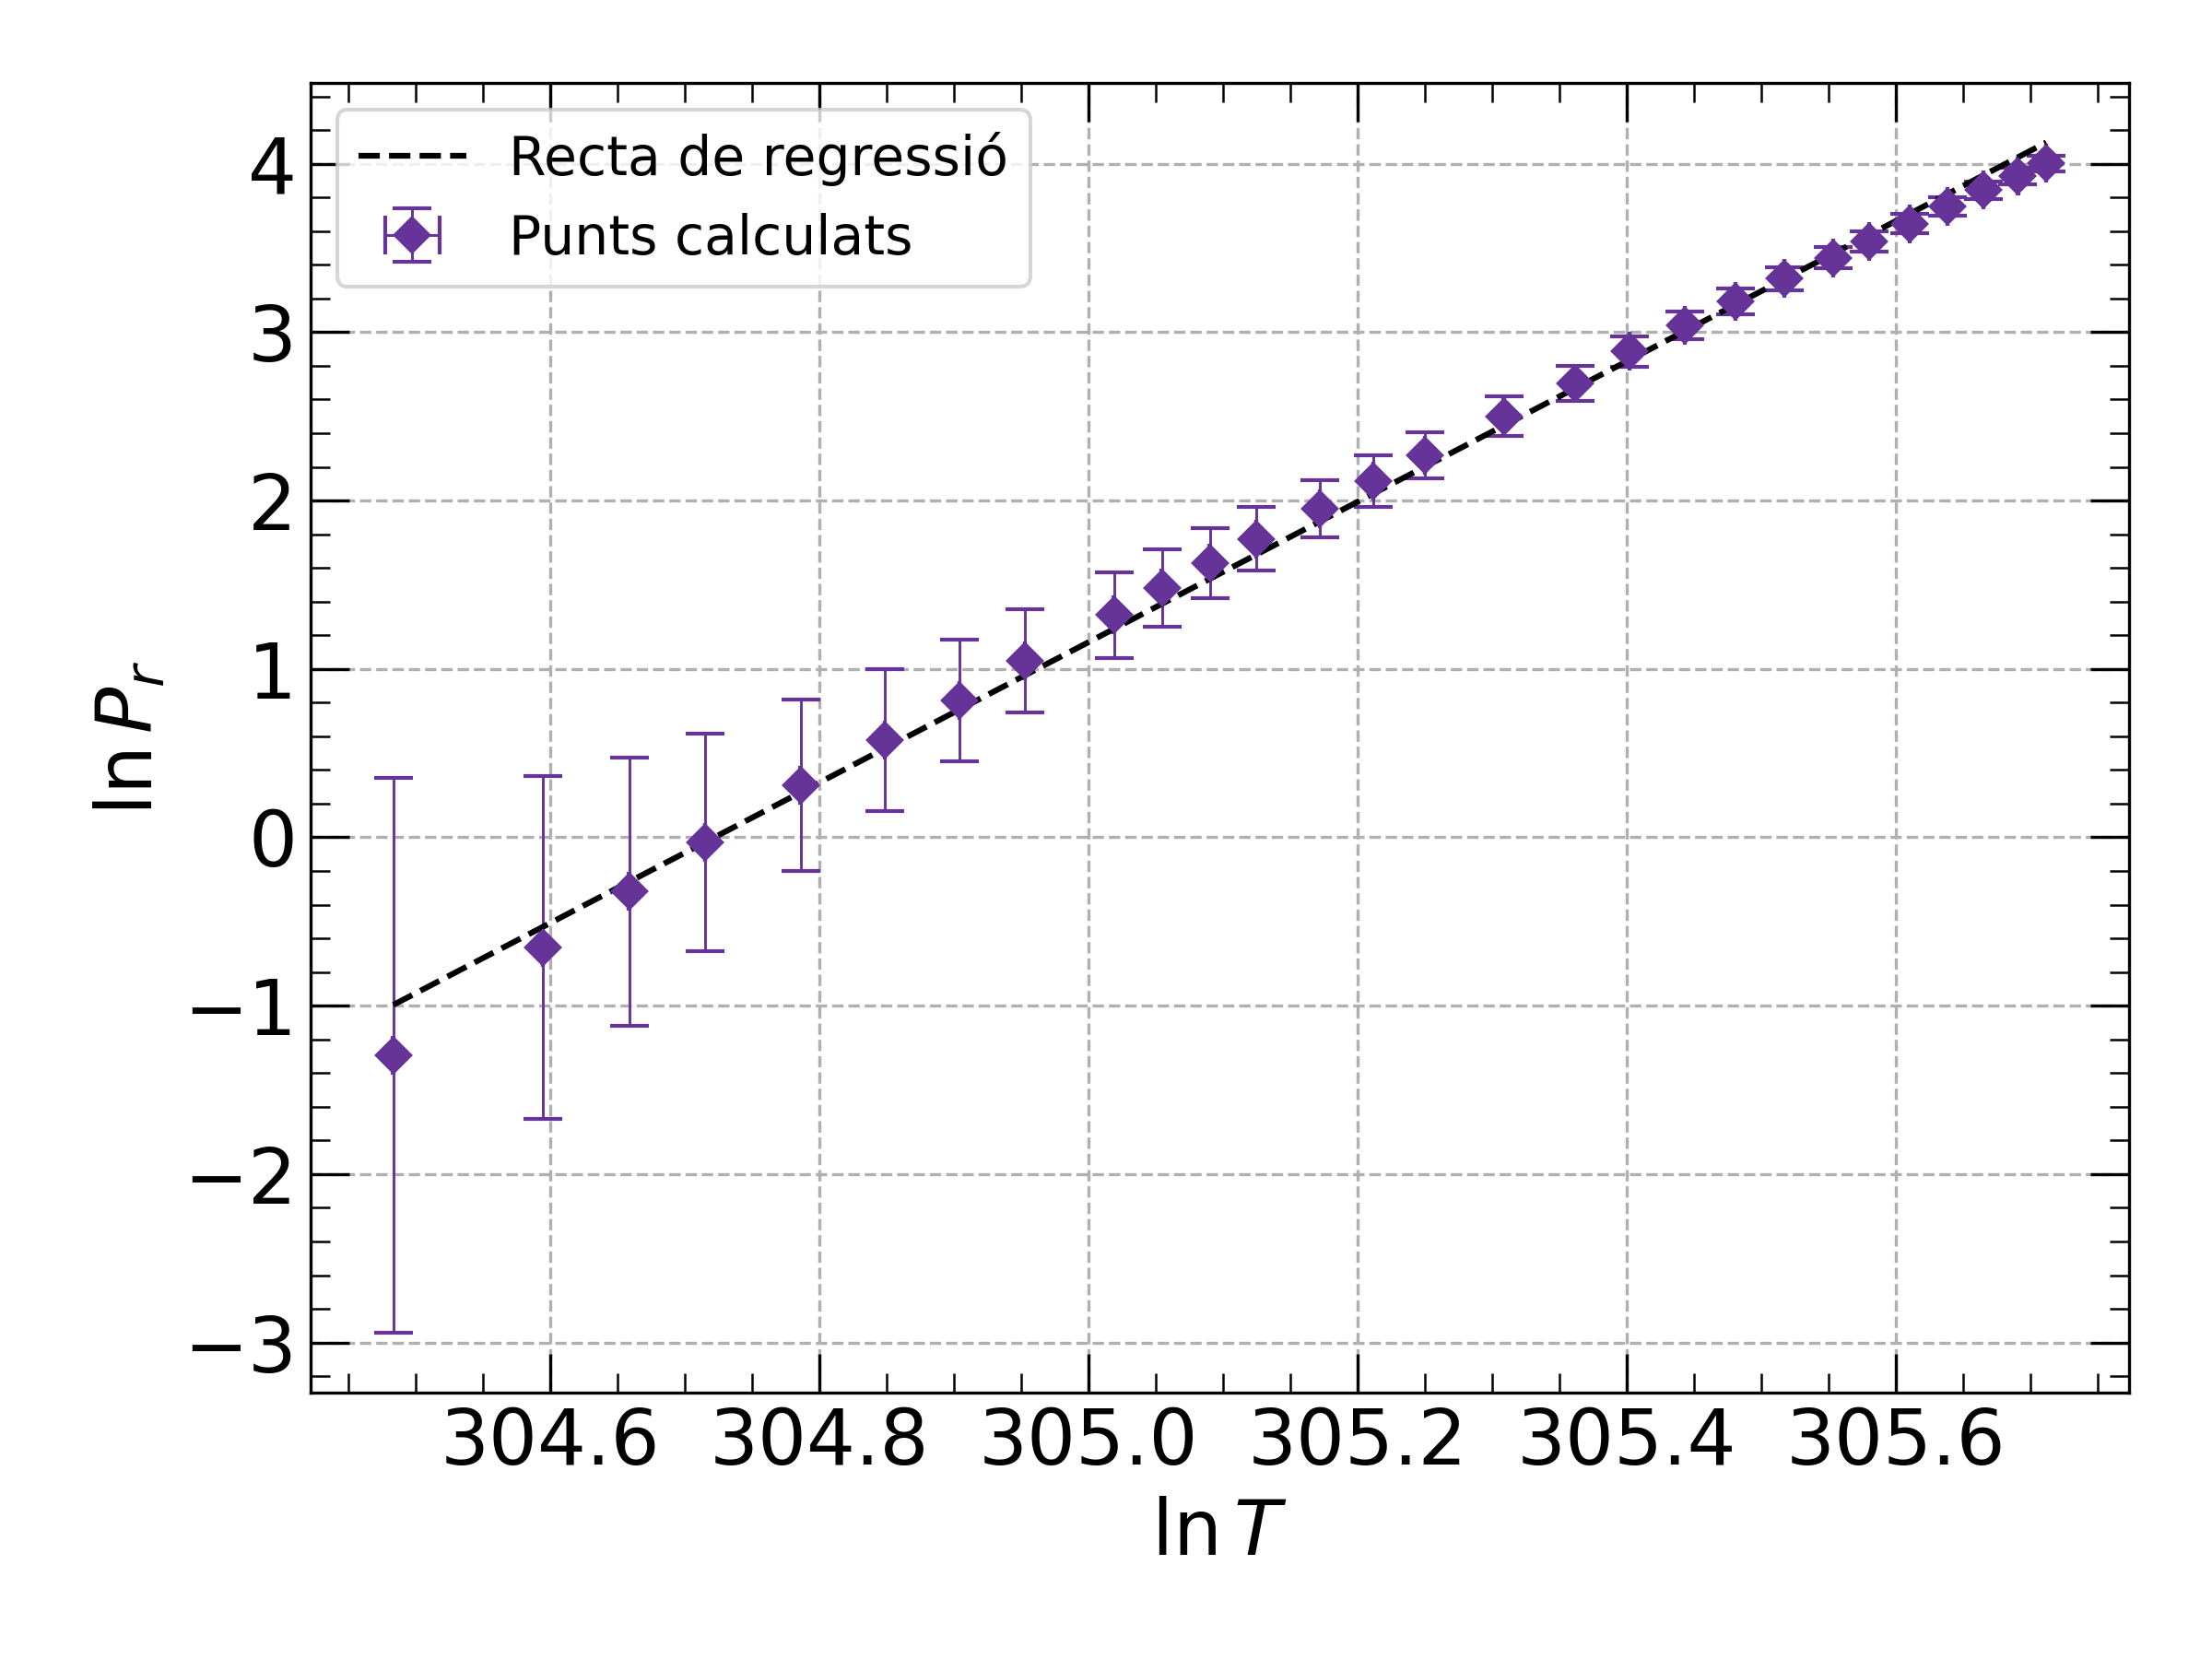
\includegraphics[width=\linewidth]{../../graphs/practica_Ib/plots/lnp_rad_vs_ln_T.png}
  \captionof{figure}{\footnotesize{Representació i regressió lineal ($y=ax+b)$ de $\ln{P_{\text{r}}}$ vs. $\ln{T}$ per a les dades de la segona regió. No s'han tingut en compte els primers 4 punts pertanyents a la regió (veure Annex). Coeficients de regressió: \(a = 4,17\pm0,05\), \(b = -1270\pm15\). Regressió amb un coeficient de $r^2=0,996$.}}
  \label{fig:lnP_rad_vs_ln_T}
\end{Figura}
Comparant amb l'Equació \eqref{ln_Stefan_Boltzmann} el pendent d'aquesta regressió hauria de ser de 4. Però, com es pot veure de les dades de la regressió, aquest valor teòric no entra dins de les incerteses. Aquesta discrepància pot venir de la contribució de la convecció, que pot estar aportant valors significatius a la potència emesa per la bombeta, o per la forma de mesurar aquest conjunt de dades, és a dir, per la poca precisió de les eines fetes servir al laboratori. Aquests errors experimentals es veuen amplificats amb la propagació d'incerteses, fet que s'arriba a veure tant a la Figura \ref{fig:lnP_rad_vs_ln_T} com comparant-la amb la Figura \ref{outliers} de l'Annex (sense eliminar outliers). Una darrera font d'error pot ser que aquestes dades amb tanta desviació pertanyen al conjunt de mesures que se situen al rang de temperatures on al laboratori realitzem el pas de corrent continu a corrent altern, dos aparells de mesura que poden tenir sensibilitat diferent.\\\\
És possible preparar una experiència que ens permeti reduir significativament no només aquests errors, sinó també reduir fins a un valor negligible les contribucions de la convecció per a poder considerar només la de la radiació als nostres càlculs. Per a fer això s'hauria de repetir l'experiència amb la bombeta en un espai on puguem fer el buit. Traient l'aire de l'entorn de la bombeta reduiria significativament l'efecte de convecció.
\subsection{Mesura directa}
A partir dels valors mesurats de forma directa de la radiació obtenim la Figura \ref{fig:rad_vs_T}, on s'observa un comportament creixent similar a un polinomi de quart grau. El sensor de radiació mesura en mV, calibrat de forma que el voltatge mesurat i la potència de radiació rebuda pel sensor són iguals \cite{PASCO}. El sensor rep la radiació que entra de forma frontal per un forat, per tant, de tota la radiació que emet la bombeta el sensor només és capaç de rebre una petita part corresponent a la seva àrea. Per aquest motiu, a la Figura \ref{fig:rad_vs_T} s'observa que el valor de la potència mesurada és petit. Però, tot i mesurar valors més petits que els que irradia la bombeta, la dependència amb la temperatura encara compleix la llei d'Stefan-Boltzmann.\\\\
A partir d'un ajust polinòmic podem calcular el valor del coeficient i del grau que segueix la radiació en funció de la temperatura. Els valors d'aquest ajust s'observen també a la Figura \ref{fig:rad_vs_T}.\\\\
Notem com, tot i no entrar dins de la incertesa, els resultats obtinguts amb aquest mètode són molt propers la corba predita per l'Equació \eqref{Stefan_Boltzmann}. Podem aplicar una forma alternativa de calcular aquest valor de l'exponent, aplicant logaritme com s'ha fet a l'apartat anterior. Seguint els mateixos passos obtenim les dades que s'observen a la Figura \ref{fig:ln_rad_vs_ln_T}, juntament amb les dades de la regressió. 
\begin{Figura}
  \centering
  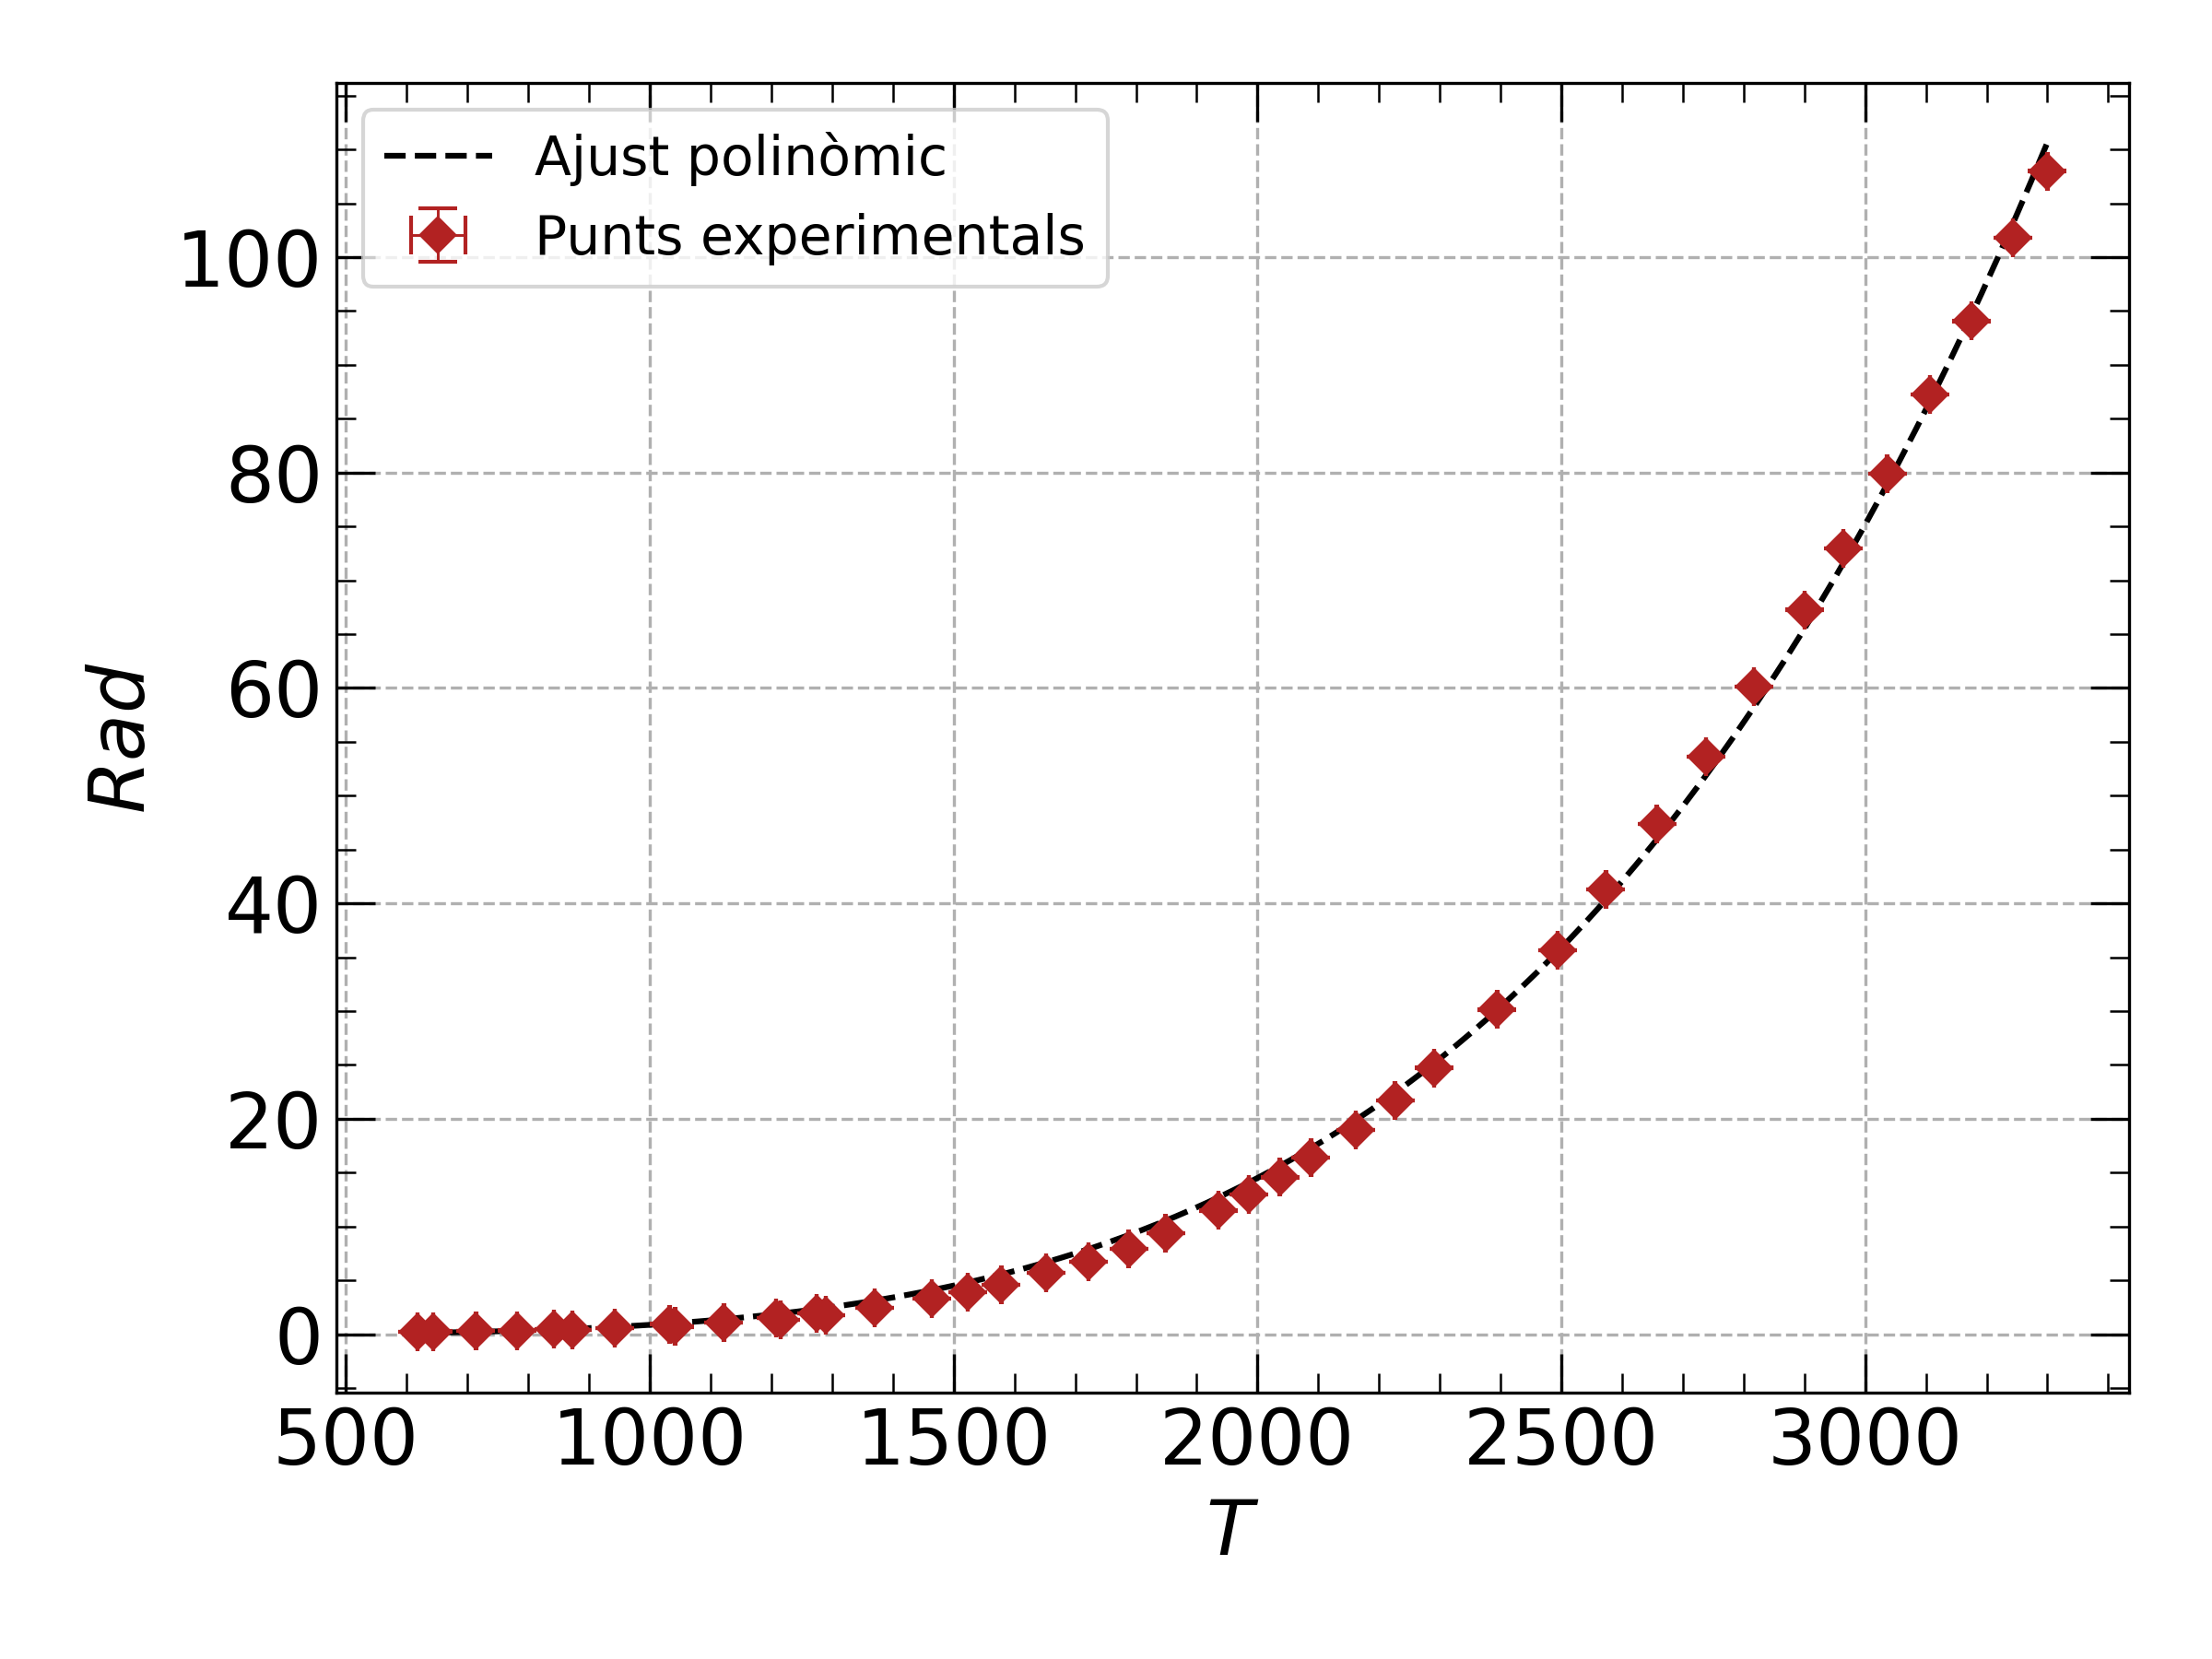
\includegraphics[width=\linewidth]{../../graphs/practica_Ib/plots/T_vs_Rad.png}
  \captionof{figure}{\footnotesize{Representació i regressió polinòmica ($y=ax^b$) de $Rad$ vs. $T$. S'indiquen les unitats de $Rad$ en W i no en V en seguir el sensor una relació un a un entre les dues unitats. Coeficients de regressió: \(a = (0,57\pm0,16)\cdot10^{-17}\,\text{W}/\text{K}^4\), $b=4,06\pm0,04$. Regressió amb un coeficient de $r^2=0,999$.}}
  \label{fig:rad_vs_T}
\end{Figura}
\begin{Figura}
  \centering
  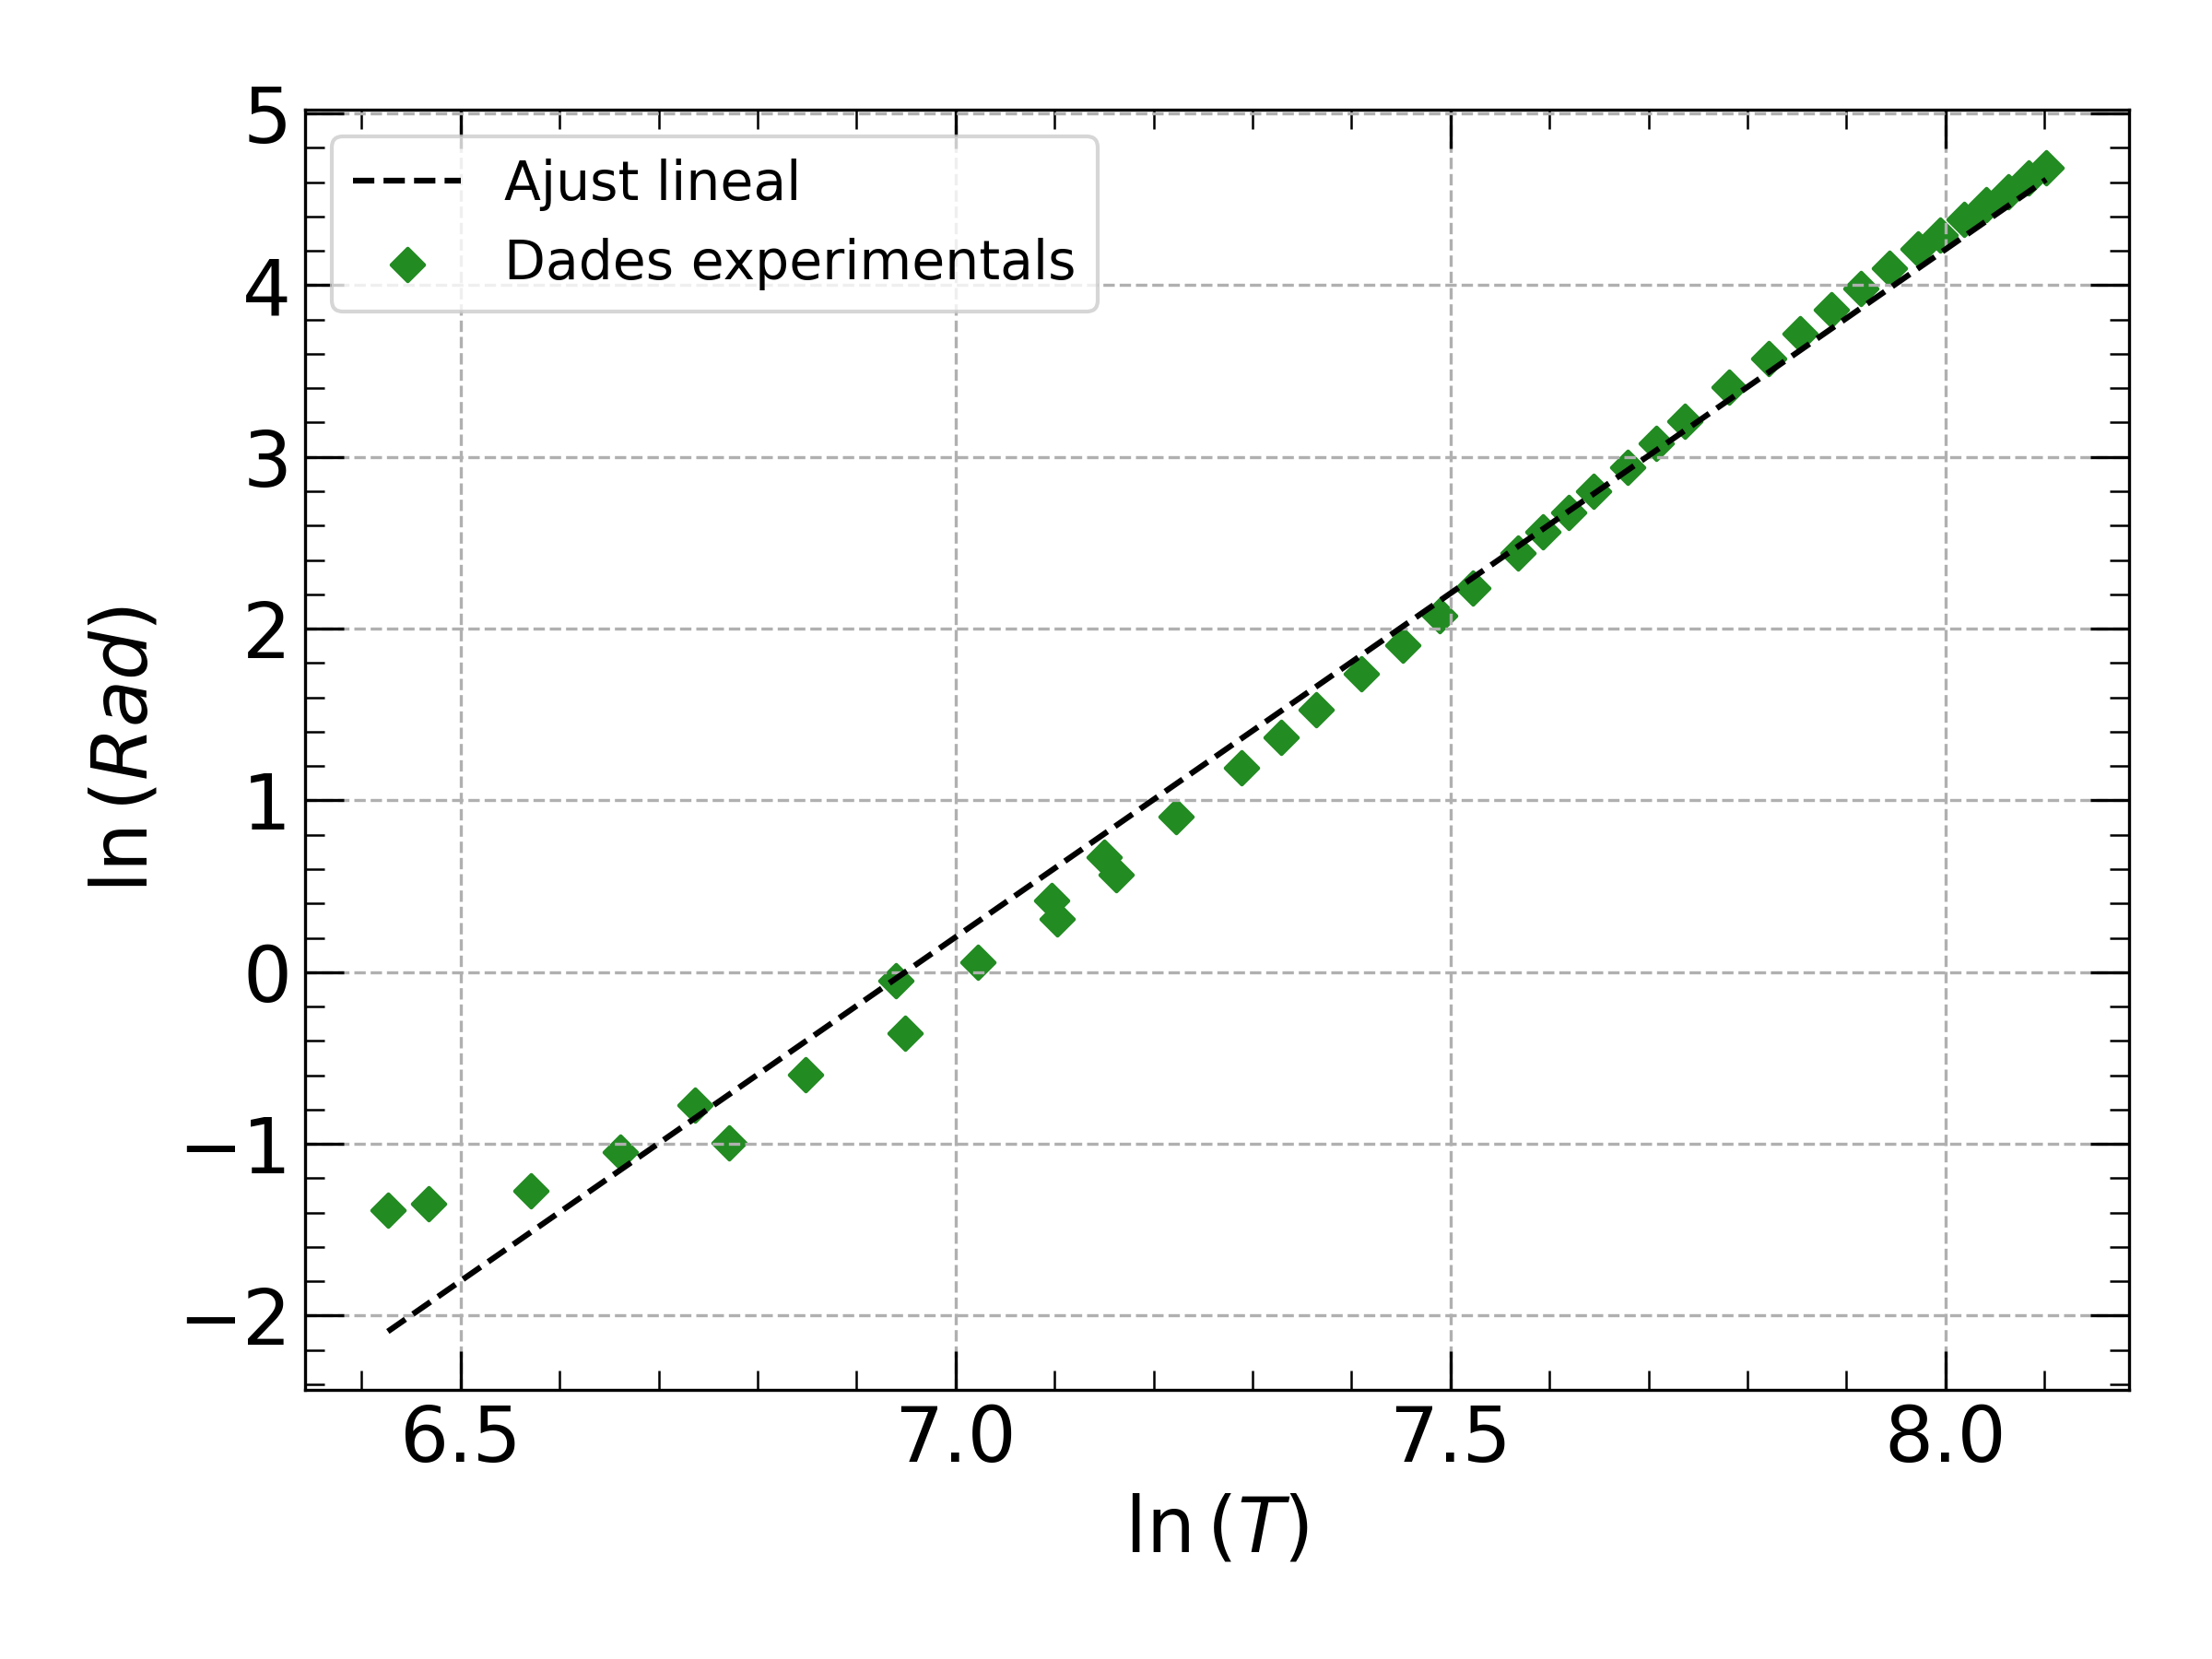
\includegraphics[width=\linewidth]{../../graphs/practica_Ib/plots/ln_T_vs_ln_Rad.png}
  \captionof{figure}{\footnotesize{Representació i regressió lineal ($y=ax+b$) de $\ln{Rad}$ vs. $\ln{T}$. Coeficients de regressió: $a=4,00\pm0,07$, $b=-34,1\pm0,5$. Regressió amb un coeficient de $r^2=0,989$.}}
  \label{fig:ln_rad_vs_ln_T}
\end{Figura}
Tot i obtenir un ajust menys ideal de les dades, obtenim un valor de l'exponent el qual sí que permet al valor teòric entrar dins la incertesa. Aquesta irregularitat de les dades del principi de la Figura \ref{fig:rad_vs_T} pot tenir origen a la precisió del instrument de mesura utilitzat a baixa temperatura, que es veu accentuat en aplicar logaritme.
\section{Conclusions}
Al llarg d'aquesta pràctica, a partir de mesures directes i indirectes de la potència de la radiació d'una bombeta de tungstè, hem comprovat com la propagació de la calor esdevé a través de diferents mecanismes alhora.\\\\
Per al nostre sistema (no aïllat de l'entorn) la potència subministrada en forma d'electricitat es dissipa en forma de calor a partir de la radiació i la convecció. Les contribucions de totes dues formes de transport varien segons el rang de temperatura en què es trobi la bombeta, però hem pogut comprovar que sempre actuen alhora. En un rang baix de temperatura respecte a la temperatura ambient la contribució més gran prové de la convecció, ja que es va escalfant l'aire al voltant de la bombeta seguint l'equació de calor de Newton i que la contribució de l'equació de Stefan-Boltzmann és petita a causa de $\sigma_{\text{SB}}$. A mesura que augmenta la temperatura aquesta contribució de la convecció es veu opacada per la contribució de la radiació. Això és deu al creixement a la quarta potència amb la temperatura, segons la llei de Stefan-Boltzmann. A partir de mesures indirectes de la potència provinent de la radiació de la bombeta hem comprovat aquest creixement polinòmic de quart grau, però, també s'ha observat com la contribució per convecció no desapareix i produeix error als resultats obtinguts.\\\\
Per a comprovar de forma directa que es compleix la llei de Stefan-Boltzmann fem servir les mesures directes de la radiació emesa per la bombeta. Amb aquestes dades s'ha posat de manifest que la radiació compleix aquesta llei. En aquest cas els resultats han sigut més coherents que els calculats de forma indirecta a partir de la potència subministrada, ja que no troben dependència amb el procés de convecció. Per a poder reproduir aquests resultats amb el mètode de mesura indirecta caldria estudiar un sistema que permeti menysprear la calor dissipada en forma de convecció, com per exemple realitzar aquestes mateixes mesures a una cambra de buit.
\section{Annex}
\subsection{Outliers}
Per a realitzar la Figura \ref{fig:ln_rad_vs_ln_T} i la seva respectiva regressió lineal s'han exclòs els primers quatre punts experimentals. Es consideren aquests punts com a outliers a causa de les seves evidents desviacions i a la recta i els valors alts d'error experimental. Com s'indica la text principal, un altre motiu per a tractar-los d'outliers és que pertanyen al rang de mesures propi de la intersecció de mesures DC i AC. A la Figura \ref{outliers} es pot observar com queda la Figura \ref{fig:lnP_rad_vs_ln_T} i els valors de regressió sense eliminar els outliers.
\begin{Figura}
  \centering
  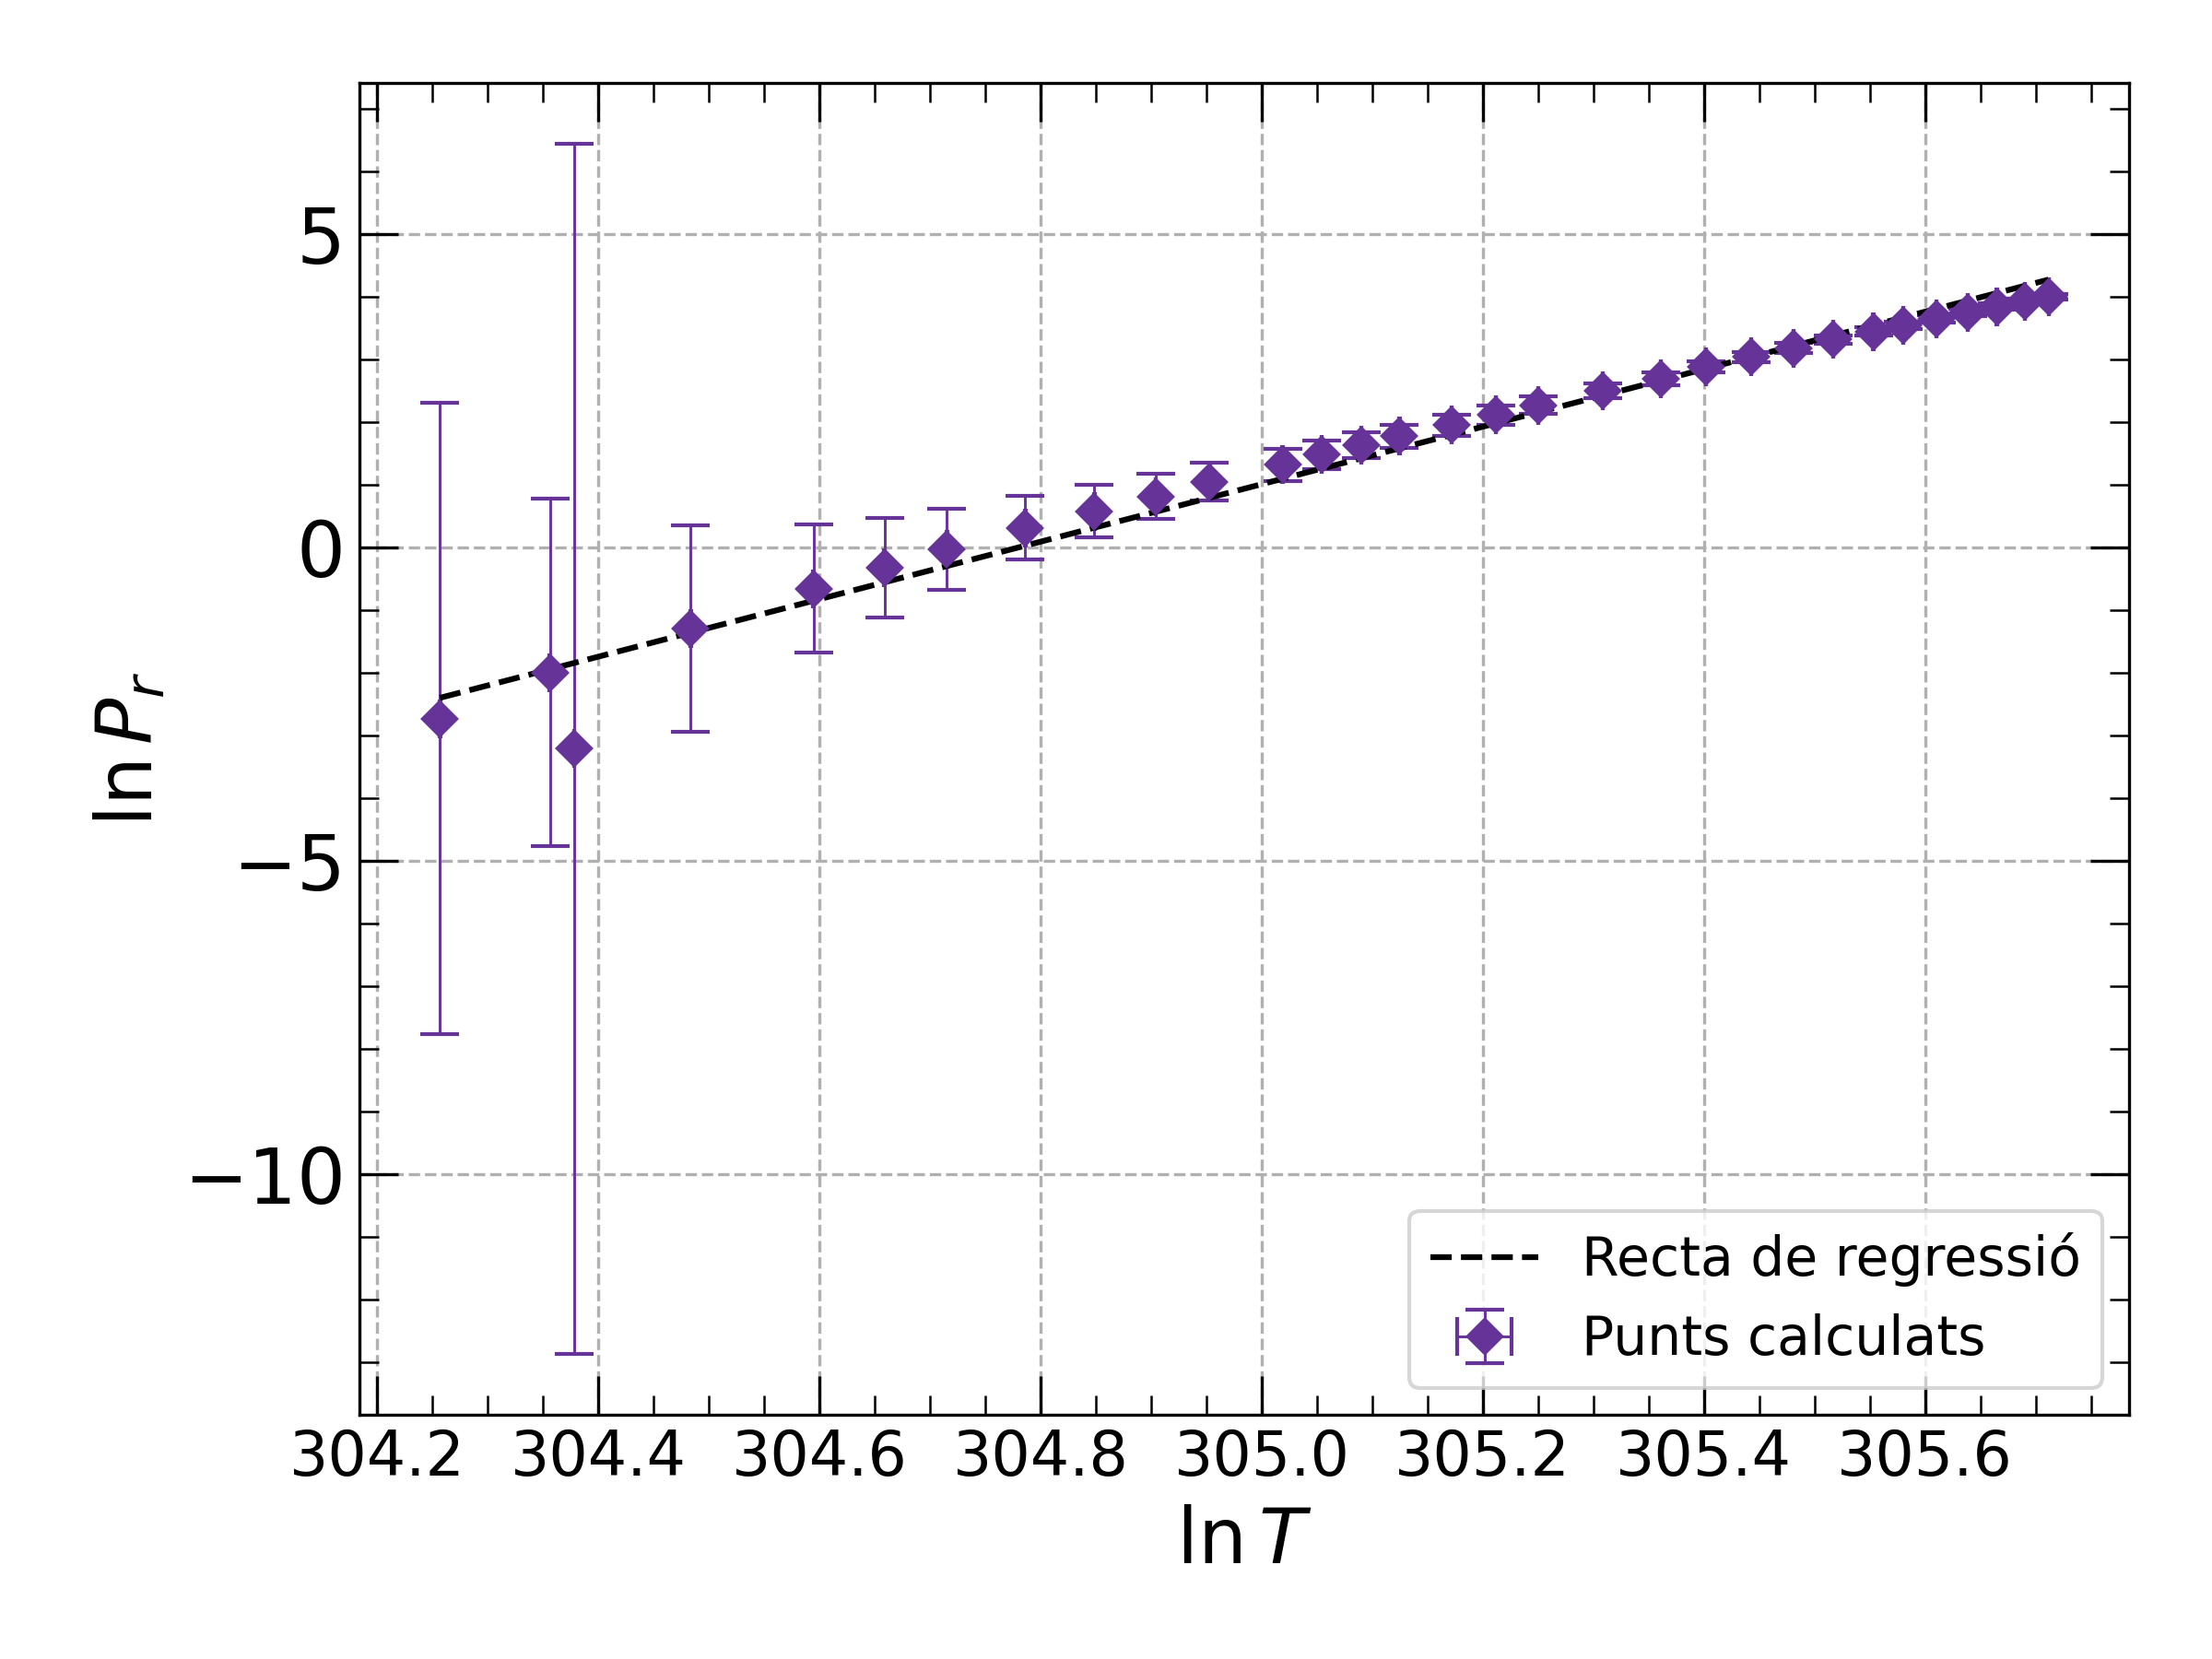
\includegraphics[width=\linewidth]{../../graphs/practica_Ib/plots/outliers.png}
  \captionof{figure}{\footnotesize{Representació i regressió lineal ($y=ax+b$) de $\ln{P_{\text{r}}}$ vs $\ln{T}$ per a les dades de la segona regió sense treure outliers. Coeficients de regressió: $a=4,59\pm0,13$, $b=(-14,0\pm0,4)\cdot10^{2}$.}}
  \label{outliers}
\end{Figura}

\subsection{Càlcul d'incerteses}
Per a calcular la incertesa dels valors mesurats directament al laboratori s'ha fet servir la desviació estàndard de la mostra obtinguda de cada valor mesurat. Juntament amb la incertesa instrumental, calculem la incertesa de cada mesura com
\begin{equation*}
    u(x_i) = \sqrt{ s_{\text{est}}^2(x_i) + s_{\text{ins}}^2}
\end{equation*}
on $s_{\text{est}}$ és la desviació estàndard, $s_{\text{ins}}$ és la incertesa instrumental i $x_i$ és la variable $i$-èssima mesurada.\\\\
Per a calcular la incertesa de magnituds derivades de les variables mesurades, s'ha fet servir la propagació d'incerteses, calculada com
\begin{equation*}
    u^2(y) = \sum_{i = 1}^{n} \left( \frac{\partial y}{\partial{x_i}} u(x_i)\right)^2
\end{equation*}
on $y$ és una funció tal que $y = y(x_1,...,x_n)$.\\\\
Per a calcular els errors de les regressions s'ha fet servir la funció \texttt{curve\_fit} de la llibreria \texttt{scipy.optimize} de Python. Per a calcular els coeficients de regressió $r^2$ s'ha aplicat el mètode de mínims quadrats, també amb Python.
\subsection{Mesures experimentals}
\renewcommand{\arraystretch}{1.35}
En aquest subapartat es deixen les dades experimentals de les mesures fetes al laboratori (Taula \ref{tau:DC} i Taula \ref{tau:AC}) i de les magnituds derivades (Taula \ref{tau:DC_calculades} i Taula \ref{tau:AC_calculades}).
\begin{Figura}
  \centering
  \captionof{table}{\footnotesize{Dades mesurades amb una font de corrent DC. Mesures preses en un rang de \(0\,\text{V}\) a \(24\,\text{V}\).}}
  \resizebox{\textwidth}{!}{
    \begin{tabular}{c|c|c}
      \multirow{2}{*}{\parbox{2cm}{\centering $V$ \\($\pm0,1$) [V]}} & \multirow{2}{*}{\parbox{2.3cm}{\centering $I$ \\ ($\pm0,1$) [mA]}} & \multirow{2}{*}{\parbox{2.5cm}{\centering $Rad$ \\ ($\pm0,01$) [mV]}}\\
      & & \\
      \hline\hline
      0,0 & 0,0 & 0,21 \\
      2,0 & 32,8 & 0,25\\
      3,0 & 44,7 & 0,26 \\
      5,2 & 62,2 & 0,28 \\
      7,2 & 72,3 & 0,35 \\
      9,0 & 79,0 & 0,46 \\
      12,0 & 87,3 & 0,55 \\
      15,1 & 93,9 & 0,70 \\
      18,0 & 99,3 & 0,95 \\
      21,1 & 104,6 & 1,36 \\
      24,0 & 109,4 & 1,76 \\
    \end{tabular}
  }
  \label{tau:DC}
\end{Figura}
\renewcommand{\arraystretch}{1.35}
\begin{Figura}
  \centering
  \captionof{table}{\footnotesize{Dades mesurades amb una font de corrent AC. Mesures preses en un rang de \(10\,\text{V}\) a \(120\,\text{V}\).}}
  \resizebox{\textwidth}{!}{
    \begin{tabular}{c|c|c}
      \multirow{2}{*}{\parbox{2cm}{\centering $V$ \\($\pm0,1$) [V]}} & \multirow{2}{*}{\parbox{2.3cm}{\centering $I$ \\ ($\pm0,1$) [mA]}} & \multirow{2}{*}{\parbox{2.5cm}{\centering $Rad$ \\ ($\pm0,01$) [mV]}}\\
      & & \\
      \hline\hline
      10,3 & 85,2 & 0,37 \\
      15,2 & 95,8 & 0,95 \\
      18,0 & 101,0 & 1,17 \\
      21,3 & 106,5 & 1,52 \\
      23,9 & 110,8 & 1,95 \\
      27,8 & 116,7 & 2,47 \\
      32,1 & 123,3 & 3,29 \\
      35,0 & 127,6 & 3,92 \\
      37,9 & 131,9 & 4,62 \\
      42,0 & 137,8 & 5,67 \\
      46,0 & 143,2 & 6,72 \\
      50,0 & 148,5 & 7,95 \\
      54,2 & 154,4 & 9,38 \\
      60,2 & 162,0 & 11,48 \\
      64,0 & 167,0 & 12,96 \\
      68,0 & 172,0 & 14,56 \\
      72,2 & 177,2 & 16,42 \\
      78,2 & 184,1 & 18,94 \\
      84,0 & 190,9 & 21,71 \\
      90,1 & 197,9 & 24,74 \\
      100,3 & 209,1 & 30,14 \\
      110,4 & 219,5 & 35,67 \\
      120,6 & 231,1 & 41,27 \\
      130,4 & 240,8 & 47,39 \\
      140,3 & 250,3 & 53,62 \\
      150,6 & 260,0 & 60,12 \\
      161,2 & 269,2 & 67,26 \\
      169,9 & 276,8 & 72,94 \\
      180,0 & 285,3 & 79,92 \\
      190,4 & 294,0 & 87,23 \\
      200,7 & 302,4 & 94,06 \\
      210,7 & 310,0 & 101,77 \\
      219,7 & 317,0 & 108,00 \\
    \end{tabular}
    }
  \label{tau:AC}
\end{Figura}
\renewcommand{\arraystretch}{1.48}
\begin{Figura}
  \centering
  \captionof{table}{\footnotesize{Dades calculades a partir de les mesures fetes amb una font de corrent AC.}}
  \resizebox{\textwidth}{!}{
    \begin{tabular}{c|c|c}
      \multirow{2}{*}{\parbox{2cm}{\centering $R$ \\ ($\cdot 10^{-3}$) [$\Omega$]}} & \multirow{2}{*}{\parbox{2.3cm}{\centering $T$ \\ ($\pm0,2$) [K]}} & \multirow{2}{*}{\parbox{2.5cm}{\centering $P_{\text{e}}$ \\ ($\cdot 10^{-1}$) [W] }}\\
       & & \\
      \hline\hline
      $120092,0 \pm 1,2$ & $872,2$ & $8,78 \pm 0,09$ \\ 
      $157863,9 \pm 1,0$ & $1032,4$ & $14,56 \pm 0,10$ \\ 
      $177417,8 \pm 1,0$ & $1115,4$ & $18,18 \pm 0,10$ \\ 
      $199200,0 \pm 0,9$ & $1207,8$ & $22,68 \pm 0,11$ \\ 
      $214904,0 \pm 0,9$ & $1274,5$ & $26,48 \pm 0,11$ \\ 
      $237417,7 \pm 0,9$ & $1370,0$ & $32,44 \pm 0,12$ \\ 
      $259540,6 \pm 0,8$ & $1463,9$ & $39,58 \pm 0,13$ \\ 
      $273494,7 \pm 0,8$ & $1523,1$ & $44,66 \pm 0,13$ \\ 
      $286538,9 \pm 0,8$ & $1578,4$ & $49,99 \pm 0,14$ \\ 
      $303989,6 \pm 0,7$ & $1652,5$ & $57,88 \pm 0,14$ \\ 
      $320429,1 \pm 0,7$ & $1722,2$ & $65,87 \pm 0,15$ \\ 
      $335900,3 \pm 0,7$ & $1787,9$ & $74,25 \pm 0,16$ \\ 
      $350236,3 \pm 0,6$ & $1848,7$ & $83,68 \pm 0,16$ \\ 
      $370804,9 \pm 0,6$ & $1936,0$ & $97,52 \pm 0,17$ \\ 
      $999200,0 \pm 1,6$ & $4602,3$ & $40,96 \pm 0,09$ \\ 
      $394548,8 \pm 0,6$ & $2036,7$ & $116,96 \pm 0,18$ \\ 
      $406649,2 \pm 0,6$ & $2088,1$ & $127,94 \pm 0,19$ \\ 
      $423969,1 \pm 0,5$ & $2161,5$ & $144,0 \pm 0,2$ \\ 
      $439221,0 \pm 0,5$ & $2226,3$ & $160,4 \pm 0,2$ \\ 
      $454480,4 \pm 0,5$ & $2291,0$ & $178,3 \pm 0,2$ \\ 
      $478874,8 \pm 0,5$ & $2394,5$ & $209,7 \pm 0,2$ \\ 
      $502161,3 \pm 0,5$ & $2493,3$ & $242,3 \pm 0,3$ \\ 
      $521052,0 \pm 0,4$ & $2573,5$ & $278,7 \pm 0,3$ \\ 
      $540728,2 \pm 0,4$ & $2657,0$ & $314,0 \pm 0,3$ \\ 
      $559727,4 \pm 0,4$ & $2737,6$ & $351,2 \pm 0,3$ \\ 
      $578430,8 \pm 0,4$ & $2816,9$ & $391,6 \pm 0,3$ \\ 
      $598011,3 \pm 0,4$ & $2900,0$ & $434,0 \pm 0,3$ \\ 
      $613000,6 \pm 0,4$ & $2963,6$ & $470,3 \pm 0,3$ \\ 
      $630114,8 \pm 0,4$ & $3036,2$ & $513,5 \pm 0,3$ \\ 
      $646819,0 \pm 0,3$ & $3107,1$ & $559,8 \pm 0,4$ \\ 
      $662890,5 \pm 0,3$ & $3175,3$ & $606,9 \pm 0,4$ \\ 
      $678877,4 \pm 0,3$ & $3243,1$ & $653,2 \pm 0,4$ \\ 
      $692259,9 \pm 0,3$ & $3299,9$ & $696,5 \pm 0,4$ \\ 
    \end{tabular}
    }
  \label{tau:AC_calculades}
\end{Figura}
\renewcommand{\arraystretch}{1.48}
\begin{Figura}
  \centering
  \captionof{table}{\footnotesize{Dades calculades a partir de les mesures fetes amb una font de corrent DC.}}
  \resizebox{\textwidth}{!}{
    \begin{tabular}{c|c|c}
      \multirow{2}{*}{\parbox{2cm}{\centering $R$ \\ ($\cdot 10^{-2}$) [$\Omega$]}} & \multirow{2}{*}{\parbox{2.3cm}{\centering $T$ \\ ($\pm0,2$) [K]}} & \multirow{2}{*}{\parbox{2.5cm}{\centering $P_{\text{e}}$ \\ ($\cdot 10^{-2}$) [W] }}\\
       & & \\
      \hline\hline
      $6017,6 \pm 0,3$ & $617,9$ & $6,56 \pm 0,3$ \\ 
      $6631,4 \pm 0,2$ & $644,0$ & $13,41 \pm 0,5$ \\ 
      $8280,1 \pm 0,2$ & $714,0 $ & $32,3 \pm 0,6$ \\ 
      $9878,5 \pm 0,1$ & $781,8$ & $52,1 \pm 0,7$ \\ 
      $11312,4 \pm 0,1$ & $842,6$ & $71,1 \pm 0,8$ \\ 
      $13665,7 \pm 0,1$ & $942,5$ & $104,8 \pm 0,9$ \\ 
      $16000,9 \pm 0,1$ & $1041,5$ & $141,8 \pm 0,1$ \\ 
      $18046,9 \pm 0,1$ & $1128,4$ & $178,7 \pm 1,0$ \\ 
      $20092,1 \pm 0,1$ & $1215,1$ & $220,7 \pm 1,1$ \\ 
      $21857,8 \pm 0,1$ & $1290,1$ & $262,6 \pm 1,1$ \\ 
    \end{tabular}
  }
  \label{tau:DC_calculades}
\end{Figura}
\end{multicols}
\bibliographystyle{plain} 
\bibliography{referencies_Ib.bib}
\end{document}